% Options for packages loaded elsewhere
\PassOptionsToPackage{unicode}{hyperref}
\PassOptionsToPackage{hyphens}{url}
\PassOptionsToPackage{dvipsnames,svgnames,x11names}{xcolor}
%
\documentclass[
  letterpaper,
  DIV=11,
  numbers=noendperiod]{scrartcl}

\usepackage{amsmath,amssymb}
\usepackage{iftex}
\ifPDFTeX
  \usepackage[T1]{fontenc}
  \usepackage[utf8]{inputenc}
  \usepackage{textcomp} % provide euro and other symbols
\else % if luatex or xetex
  \usepackage{unicode-math}
  \defaultfontfeatures{Scale=MatchLowercase}
  \defaultfontfeatures[\rmfamily]{Ligatures=TeX,Scale=1}
\fi
\usepackage{lmodern}
\ifPDFTeX\else  
    % xetex/luatex font selection
\fi
%% Support for zero-width non-joiner characters.
\makeatletter
\def\zerowidthnonjoiner{%
  % Prevent ligatures and adjust kerning, but still support hyphenating.
  \texorpdfstring{%
    \TextOrMath{\nobreak\discretionary{-}{}{\kern.03em}%
      \ifvmode\else\nobreak\hskip\z@skip\fi}{}%
  }{}%
}
\makeatother
\ifPDFTeX
  \DeclareUnicodeCharacter{200C}{\zerowidthnonjoiner}
\else
  \catcode`^^^^200c=\active
  \protected\def ^^^^200c{\zerowidthnonjoiner}
\fi
%% End of ZWNJ support
% Use upquote if available, for straight quotes in verbatim environments
\IfFileExists{upquote.sty}{\usepackage{upquote}}{}
\IfFileExists{microtype.sty}{% use microtype if available
  \usepackage[]{microtype}
  \UseMicrotypeSet[protrusion]{basicmath} % disable protrusion for tt fonts
}{}
\makeatletter
\@ifundefined{KOMAClassName}{% if non-KOMA class
  \IfFileExists{parskip.sty}{%
    \usepackage{parskip}
  }{% else
    \setlength{\parindent}{0pt}
    \setlength{\parskip}{6pt plus 2pt minus 1pt}}
}{% if KOMA class
  \KOMAoptions{parskip=half}}
\makeatother
\usepackage{xcolor}
\setlength{\emergencystretch}{3em} % prevent overfull lines
\setcounter{secnumdepth}{5}
% Make \paragraph and \subparagraph free-standing
\makeatletter
\ifx\paragraph\undefined\else
  \let\oldparagraph\paragraph
  \renewcommand{\paragraph}{
    \@ifstar
      \xxxParagraphStar
      \xxxParagraphNoStar
  }
  \newcommand{\xxxParagraphStar}[1]{\oldparagraph*{#1}\mbox{}}
  \newcommand{\xxxParagraphNoStar}[1]{\oldparagraph{#1}\mbox{}}
\fi
\ifx\subparagraph\undefined\else
  \let\oldsubparagraph\subparagraph
  \renewcommand{\subparagraph}{
    \@ifstar
      \xxxSubParagraphStar
      \xxxSubParagraphNoStar
  }
  \newcommand{\xxxSubParagraphStar}[1]{\oldsubparagraph*{#1}\mbox{}}
  \newcommand{\xxxSubParagraphNoStar}[1]{\oldsubparagraph{#1}\mbox{}}
\fi
\makeatother


\providecommand{\tightlist}{%
  \setlength{\itemsep}{0pt}\setlength{\parskip}{0pt}}\usepackage{longtable,booktabs,array}
\usepackage{calc} % for calculating minipage widths
% Correct order of tables after \paragraph or \subparagraph
\usepackage{etoolbox}
\makeatletter
\patchcmd\longtable{\par}{\if@noskipsec\mbox{}\fi\par}{}{}
\makeatother
% Allow footnotes in longtable head/foot
\IfFileExists{footnotehyper.sty}{\usepackage{footnotehyper}}{\usepackage{footnote}}
\makesavenoteenv{longtable}
\usepackage{graphicx}
\makeatletter
\newsavebox\pandoc@box
\newcommand*\pandocbounded[1]{% scales image to fit in text height/width
  \sbox\pandoc@box{#1}%
  \Gscale@div\@tempa{\textheight}{\dimexpr\ht\pandoc@box+\dp\pandoc@box\relax}%
  \Gscale@div\@tempb{\linewidth}{\wd\pandoc@box}%
  \ifdim\@tempb\p@<\@tempa\p@\let\@tempa\@tempb\fi% select the smaller of both
  \ifdim\@tempa\p@<\p@\scalebox{\@tempa}{\usebox\pandoc@box}%
  \else\usebox{\pandoc@box}%
  \fi%
}
% Set default figure placement to htbp
\def\fps@figure{htbp}
\makeatother
% definitions for citeproc citations
\NewDocumentCommand\citeproctext{}{}
\NewDocumentCommand\citeproc{mm}{%
  \begingroup\def\citeproctext{#2}\cite{#1}\endgroup}
\makeatletter
 % allow citations to break across lines
 \let\@cite@ofmt\@firstofone
 % avoid brackets around text for \cite:
 \def\@biblabel#1{}
 \def\@cite#1#2{{#1\if@tempswa , #2\fi}}
\makeatother
\newlength{\cslhangindent}
\setlength{\cslhangindent}{1.5em}
\newlength{\csllabelwidth}
\setlength{\csllabelwidth}{3em}
\newenvironment{CSLReferences}[2] % #1 hanging-indent, #2 entry-spacing
 {\begin{list}{}{%
  \setlength{\itemindent}{0pt}
  \setlength{\leftmargin}{0pt}
  \setlength{\parsep}{0pt}
  % turn on hanging indent if param 1 is 1
  \ifodd #1
   \setlength{\leftmargin}{\cslhangindent}
   \setlength{\itemindent}{-1\cslhangindent}
  \fi
  % set entry spacing
  \setlength{\itemsep}{#2\baselineskip}}}
 {\end{list}}
\usepackage{calc}
\newcommand{\CSLBlock}[1]{\hfill\break\parbox[t]{\linewidth}{\strut\ignorespaces#1\strut}}
\newcommand{\CSLLeftMargin}[1]{\parbox[t]{\csllabelwidth}{\strut#1\strut}}
\newcommand{\CSLRightInline}[1]{\parbox[t]{\linewidth - \csllabelwidth}{\strut#1\strut}}
\newcommand{\CSLIndent}[1]{\hspace{\cslhangindent}#1}

\KOMAoption{captions}{tableheading}
\makeatletter
\@ifpackageloaded{caption}{}{\usepackage{caption}}
\AtBeginDocument{%
\ifdefined\contentsname
  \renewcommand*\contentsname{Table of contents}
\else
  \newcommand\contentsname{Table of contents}
\fi
\ifdefined\listfigurename
  \renewcommand*\listfigurename{List of Figures}
\else
  \newcommand\listfigurename{List of Figures}
\fi
\ifdefined\listtablename
  \renewcommand*\listtablename{List of Tables}
\else
  \newcommand\listtablename{List of Tables}
\fi
\ifdefined\figurename
  \renewcommand*\figurename{Figure}
\else
  \newcommand\figurename{Figure}
\fi
\ifdefined\tablename
  \renewcommand*\tablename{Table}
\else
  \newcommand\tablename{Table}
\fi
}
\@ifpackageloaded{float}{}{\usepackage{float}}
\floatstyle{ruled}
\@ifundefined{c@chapter}{\newfloat{codelisting}{h}{lop}}{\newfloat{codelisting}{h}{lop}[chapter]}
\floatname{codelisting}{Listing}
\newcommand*\listoflistings{\listof{codelisting}{List of Listings}}
\makeatother
\makeatletter
\makeatother
\makeatletter
\@ifpackageloaded{caption}{}{\usepackage{caption}}
\@ifpackageloaded{subcaption}{}{\usepackage{subcaption}}
\makeatother

\usepackage{bookmark}

\IfFileExists{xurl.sty}{\usepackage{xurl}}{} % add URL line breaks if available
\urlstyle{same} % disable monospaced font for URLs
\hypersetup{
  pdftitle={Algorithm Design and Theoretical Basis Description},
  pdfauthor={Krasen Samardzhiev, Barbara Metzler, Martin Fleischmann, Dani Arribas-Bel},
  colorlinks=true,
  linkcolor={blue},
  filecolor={Maroon},
  citecolor={Blue},
  urlcolor={Blue},
  pdfcreator={LaTeX via pandoc}}


\title{Algorithm Design and Theoretical Basis Description}
\usepackage{etoolbox}
\makeatletter
\providecommand{\subtitle}[1]{% add subtitle to \maketitle
  \apptocmd{\@title}{\par {\large #1 \par}}{}{}
}
\makeatother
\subtitle{Technical Note D2}
\author{Krasen Samardzhiev, Barbara Metzler, Martin Fleischmann, Dani
Arribas-Bel}
\date{}

\begin{document}
\maketitle

\renewcommand*\contentsname{Table of contents}
{
\hypersetup{linkcolor=}
\setcounter{tocdepth}{3}
\tableofcontents
}

\section{Executive summary}\label{executive-summary}

The detailed classification of urban form can provide valuable insights
into the structure of cities and towns, guide targeted policy
applications, and form the backbone of urban planning. However,
classification of this sort are scarcely available and even fewer are
detailed, scalable, and consistent while reflecting the nature of the
local data all at the same time. We often see conceptual classification,
which has a tendency to oversimplify the structure when ``zooming in'',
loosing the interest of planners and policy-makers. The classifications
developed by key members of the EuroFab project team overcome these
limitations, but are dependent on the availability of high quality data
capturing urban form, e.g.~individual buildings and related street
networks. The issue is that these are not always readily available, even
within the context of generally data-rich countries of the European
region. Therefore, there is a need to derive such classification from
suboptimal data that do not have the same qualities as, for example,
cadastre would have, but have consistency and continental coverage. This
Technical Note outlines the theoretical and methodological bases for two
models - one based on satellite-derived building footprints; and a
second, based on a direct use of Sentinel-2 visible bands. The models
aim to adress the data issues presented above, while maintaining the
quality of urban classification needed by practioners.

The first model, which we can call morphological, uses the Microsoft
Open Buildings footprints dataset of a remote-sensing origin and
predicts the classes provided by an authoritative target classification
based on cadastral data. It measures morphological variables based on
building footprints, linked to street network coming from the Overture
Maps project and uses the measurements to predict the authoritative
classification using non-linear tree-based ensemble models. The
evaluated models are trained using spatially explicit splits and are
extensively tested for a robustness of prediction in an out-of-sample
context. We further use the results of the models as an iterative
feedback loop allowing gap-filling of the original taxonomy when the
model detects urban fabric it has not seen before and is therefore not
able to reliably classify.

The second model, which we can call the AI model, works on top of
Sentinel-2 visible bands at 10 meters per pixel resolution, and aims to
provide a prediction using the foundational computer vision models,
eventually allowing deployment of a predicted time series followed-up by
yearly updates. The related work package compares three different
architectures based on a direct extraction of model embeddings,
segmentation, and classification, based on different foundational models
(SatlasPretrain for the embeddings, SatlasPretrain, Clay, and IBM/NASA's
Prithvi for segmentation, Clay for classification). To further improve
the model performance and acknowledge the effects of spatial
heterogeneity, models optionally include explicit spatial dimension
encoded via H3 grid locations. Overall, the classification approach with
regional information (H3 Level 5) yielded the best performance,
achieving both high accuracy and a reasonable balance across classes.
Additionally, this approach is computationally efficient: once the image
embeddings are generated, the downstream classification process can be
completed in just a few minutes.

\section{Theoretical basis}\label{theoretical-basis}

This report describes in detail the data, the data preprocessing, as
well as model selection, training and validation schemes. The background
section positions the research in the literature and identifies the
drawbacks of current approaches, this study aims to address. It also
provides some background on the study area - Central Europe. The data
section describes the input, output and target data for the model. The
methodology section focuses on the model selection, training and
validation approaches.

\subsection{Morphometric Classification
Homogenisation}\label{morphometric-classification-homogenisation}

The spatial layout of the physical elements of cities - its urban fabric
- affects most activities their residents undertake, from accessing
services or jobs to their social and cultural lives. Analysing the
interplay of urban form, land use, mobility and other dimensions of
human activities provides insights into how cities evolve and what
effective developmental policies should look like. Researchers in the
field of urban morphology have spend years in identifying, classifying
and analysing the variations in urban form across cities from all over
the world. A core new development, powered by advancements in spatial
data science, computer vision, and open data availability, are the
methodologies created to computationally discern and analyse urban
fabric (Fleischmann et al. 2022). Taken together, these facts have
opened up the possibility of a more systematic and comprehensive
approach to the classification of urban morphological patterns, which in
turn can drive our understanding of cities (Calafiore et al. 2023;
Arribas-Bel and Fleischmann 2022).

One factor that limits the wider application of these methods is their
dependency on high-quality data, that is generally not available for
every city. For example, (Fleischmann et al. 2022; Arribas-Bel and
Fleischmann 2022) use building polygons from the respective municipal
and national mapping agencies. However, such data is not generally
available even for most high-income countries. And where available, it
can come in various formats and the data itself is not necessarily
homogenous, which makes its processing difficult. For example, official
Czechia cadastral building polygons (https://services.cuzk.cz/) come as
a GeoPackage, with no information about building age, height, type or
use. In contrast, official German building polygons, come separately for
every state , typically but not always as GML data from a WFS service,
and sometimes have extra building information. However, the definition
of building is different to Czechia and the polygon set may include
parts of tunnels, overpasses or tram lines. These definitions are even
sometimes different in the cases of cities within the same country -
i.e.~the data for Berlin and Hamburg is different from the data
available for Bremen.

EuroFab aims to address the data availability and processing issues, as
well as broaden the applicability of urban morphometrics. It does this
through the development of a predictive urban morphometric model which
uses widely available building footprints to infer structure of urban
form. The model input is calculated directly on satellite-derived
building footprints, which gives it a global scope and thus eliminates
the need the data fusion problems described above. Furthermore, it is
trained on a detailed morphometric classification derived from official
cadastre data in a large study area that covers multiple countries -
Poland, Austria, Czechia, Germany and Slovakia, i.e.~Central Europe. The
heterogeneity of urban form and planning regimes present in the study
area enables the model to distinguish a rich variety of urban patterns
and improves it generalisability.

The specific approach taken has four stages. In the first stage
morphological elements and their characteristics are calculated using
the widely available Microsoft building and Overture Maps Transportation
data. These elements are the predictor variables that the model will
use. To achieve this we develop a highly-scalable polygon and street
data pipeline, capable of calculating an exhaustive list of morphometric
characteristics. In the second stage, each element, calculated in the
first stage, is assigned a target classification label based on spatial
overlap with morphological elements from (Fleischmann and Samardzhiev
Forthcoming). (Fleischmann and Samardzhiev Forthcoming) is a
classification of urban fabrics in Central Europe based on the
highest-detail available cadastre data. Third, the data is then split
into five training and testing subsets, so that every country and every
combination of the other four countries are used as test and training
data respectively. Lastly, a series of non-linear models are trained on
each subset to predict the morphological classification of individual
elements, using a custom cross-validation scheme in order to account for
spatial leakage. Our training and testing setup emphasises evaluating
the model's ability to deal with realistic scenarios and with previously
unseen data and new urban fabric types. The best performing model is
chosen as the final production model, and retrained on the whole
dataset.

Satellite derived building footprints are becoming more widely adopted,
however, the data does not come without issues. For example, in dense
urban centres entire blocks can be delineated as individual buildings.
Given that morphology calculations rely on precise local topological
relations between neighbours, such as two buildings touching, this
problem renders a whole number of possible measurements described in
(Fleischmann, Romice, and Porta 2021) meaningless. Furthermore, this
issue affects even simpler calculations such as counting the number of
buildings within a radius or topological neighbourhood. Other issues are
that computer vision techniques sometimes miss entire buildings or
misidentify building boundaries. Therefore, any approach that uses
satellite-derived building footprints should be able to account for
these three and potentially other problems.

Implementing these stages, and further realising the potential of the
model for global application, requires the creation of novel, scalable
data processing pipelines capable of analysing hundreds of millions of
morphological elements - buildings, streets and their derivatives. Due
to their scalability, these pipelines can further be reused for other
work, outside of the immediate scope of this projects. To ensure maximum
impact and high standards, all work for this project follows open
science principles and is open-sourced on GitHub.

\subsection{AI Modelling using Satellite
Imagery}\label{ai-modelling-using-satellite-imagery}

Advancements in satellite imagery and artificial intelligence (AI) have
significantly enhanced our ability to analyze complex geospatial
datasets. Satellite imagery provides detailed information at varying
spatial and temporal scales, enabling applications that range from
analyzing individual buildings to studying entire continents. By
extracting visual and spectral data, satellite images offer insights
into ground conditions such as land cover and land use classification
(Esch et al. 2010; Ma et al. 2019; Ibrahim, Haworth, and Cheng 2020;
Huang, Zhao, and Song 2018). AI algorithms transform these data into
actionable insights by automating the analysis of vast amounts of
pixel-level information. However, many conventional AI models are
designed for specific tasks and require significant fine-tuning for new
applications.

The emergence of foundation models in geospatial AI (GeoAI) marks a
transformative shift. Unlike traditional task-specific models,
foundation models are pre-trained on large, diverse datasets and can be
adapted to multiple tasks with minimal additional training (Rolf et al.
2021). This adaptability is particularly useful in remote sensing, where
data are often complex, integrating multi-spectral and multi-temporal
information (Lu et al. 2024).

Foundation models have recently demonstrated superior performance,
especially in scenarios with limited labeled data. Transformer-based
architectures, pre-trained on extensive multispectral datasets, have
become central to GeoAI research. Notable examples include Prithvi
(Jakubik et al. 2023) and SatlasPretrain (Bastani et al. 2023), which
were trained on terabytes of imagery and millions of labeled instances.
These models have achieved state-of-the-art results in tasks such as
image classification and multi-temporal image segmentation, illustrating
their ability to address diverse and complex Earth observation
challenges.

\section{Algorithm Design}\label{algorithm-design}

\subsection{Morphometric Classification
Homogenisation}\label{morphometric-classification-homogenisation-1}

\subsubsection{Model architecture}\label{model-architecture}

The model architecture consists of the two main components: 1)
derivation of predictive variables, and 2) development of the predictive
model. Given the target of the prediction is morphological
classification, we use morphometric measurements based on the
sub-standard satellite-derived data as predictive variables, as they are
conceptually related - the original target classification is a result of
unsupervised learning on top of morphometric measurements based on
cadastral data. The model's main job is then to capture the shift of
meaning of individual characters from the original, when measured on
precise geometries, to the derived one, measured on imperfect
representation of urban form. Given the model will eventually perform a
prediction out of the sample, we further build in a logic identifying
the types of urban form it has not seen previously and ingesting then
manually in the original taxonomy, forming an iterative feedback loop.
The whole system is illustrated in Figure 1.

\begin{figure}[H]

{\centering 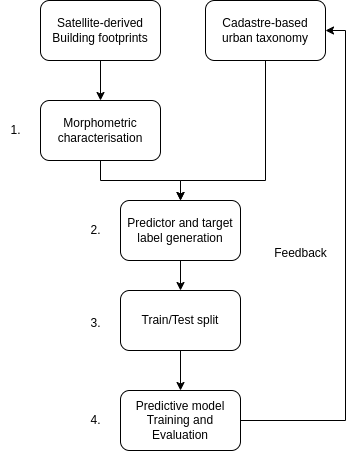
\includegraphics[width=\linewidth,height=4.16667in,keepaspectratio]{../figures/algo_design/workflow.png}

}

\caption{Project workflow}

\end{figure}%

The data preparation and model training consists of four stages. The
first and second stages cover the morphometric characterisation, which
acts as the model's predictor variables, and the target variables
generation. The third stage splits splits the whole study area into five
subsets, so that every country and every combintion of the four other
countries in the area, act as test and training data respectively. The
final stage is the model training and evaluation, aiming to minimise
spatial leakeage in the training and evaluation data, and testing the
model's performance on realistic scenarios. The full model training and
evaluation framework will be implemented using scikit-learn pipelines.

\subsubsection{Data preprocessing}\label{data-preprocessing}

\paragraph{Building preprocessing}\label{building-preprocessing}

All available Microsoft building footprints for the study area are used
for the analysis. Typically, building polygons required for
morphological studies have to be of very high quality. For example,
building polygons overlapping by a thousandth of a millimetre break
topological contiguity and therefore affect the calculation of
morphological properties, such as the ratio of shared walls, or the
number of adjacent buildings. Furthermore, even the highest quality
available software suffers from numerical precision issues which
exasperate the above problem. Another potential issue is the inclusion
of artefacts we are not directly interested in such as sheds or market
stalls. Most importantly, polygons shall represent individual buildings,
not compounds of buildings that are adjacent. The footprints used for
this study fall short of these standards. Therefore, our approach aims
to accommodate less than ideal data and methods, first by processing the
building data, and second, by adapting the morphological calculations to
account for numerical issues.

\begin{figure}[H]

{\centering 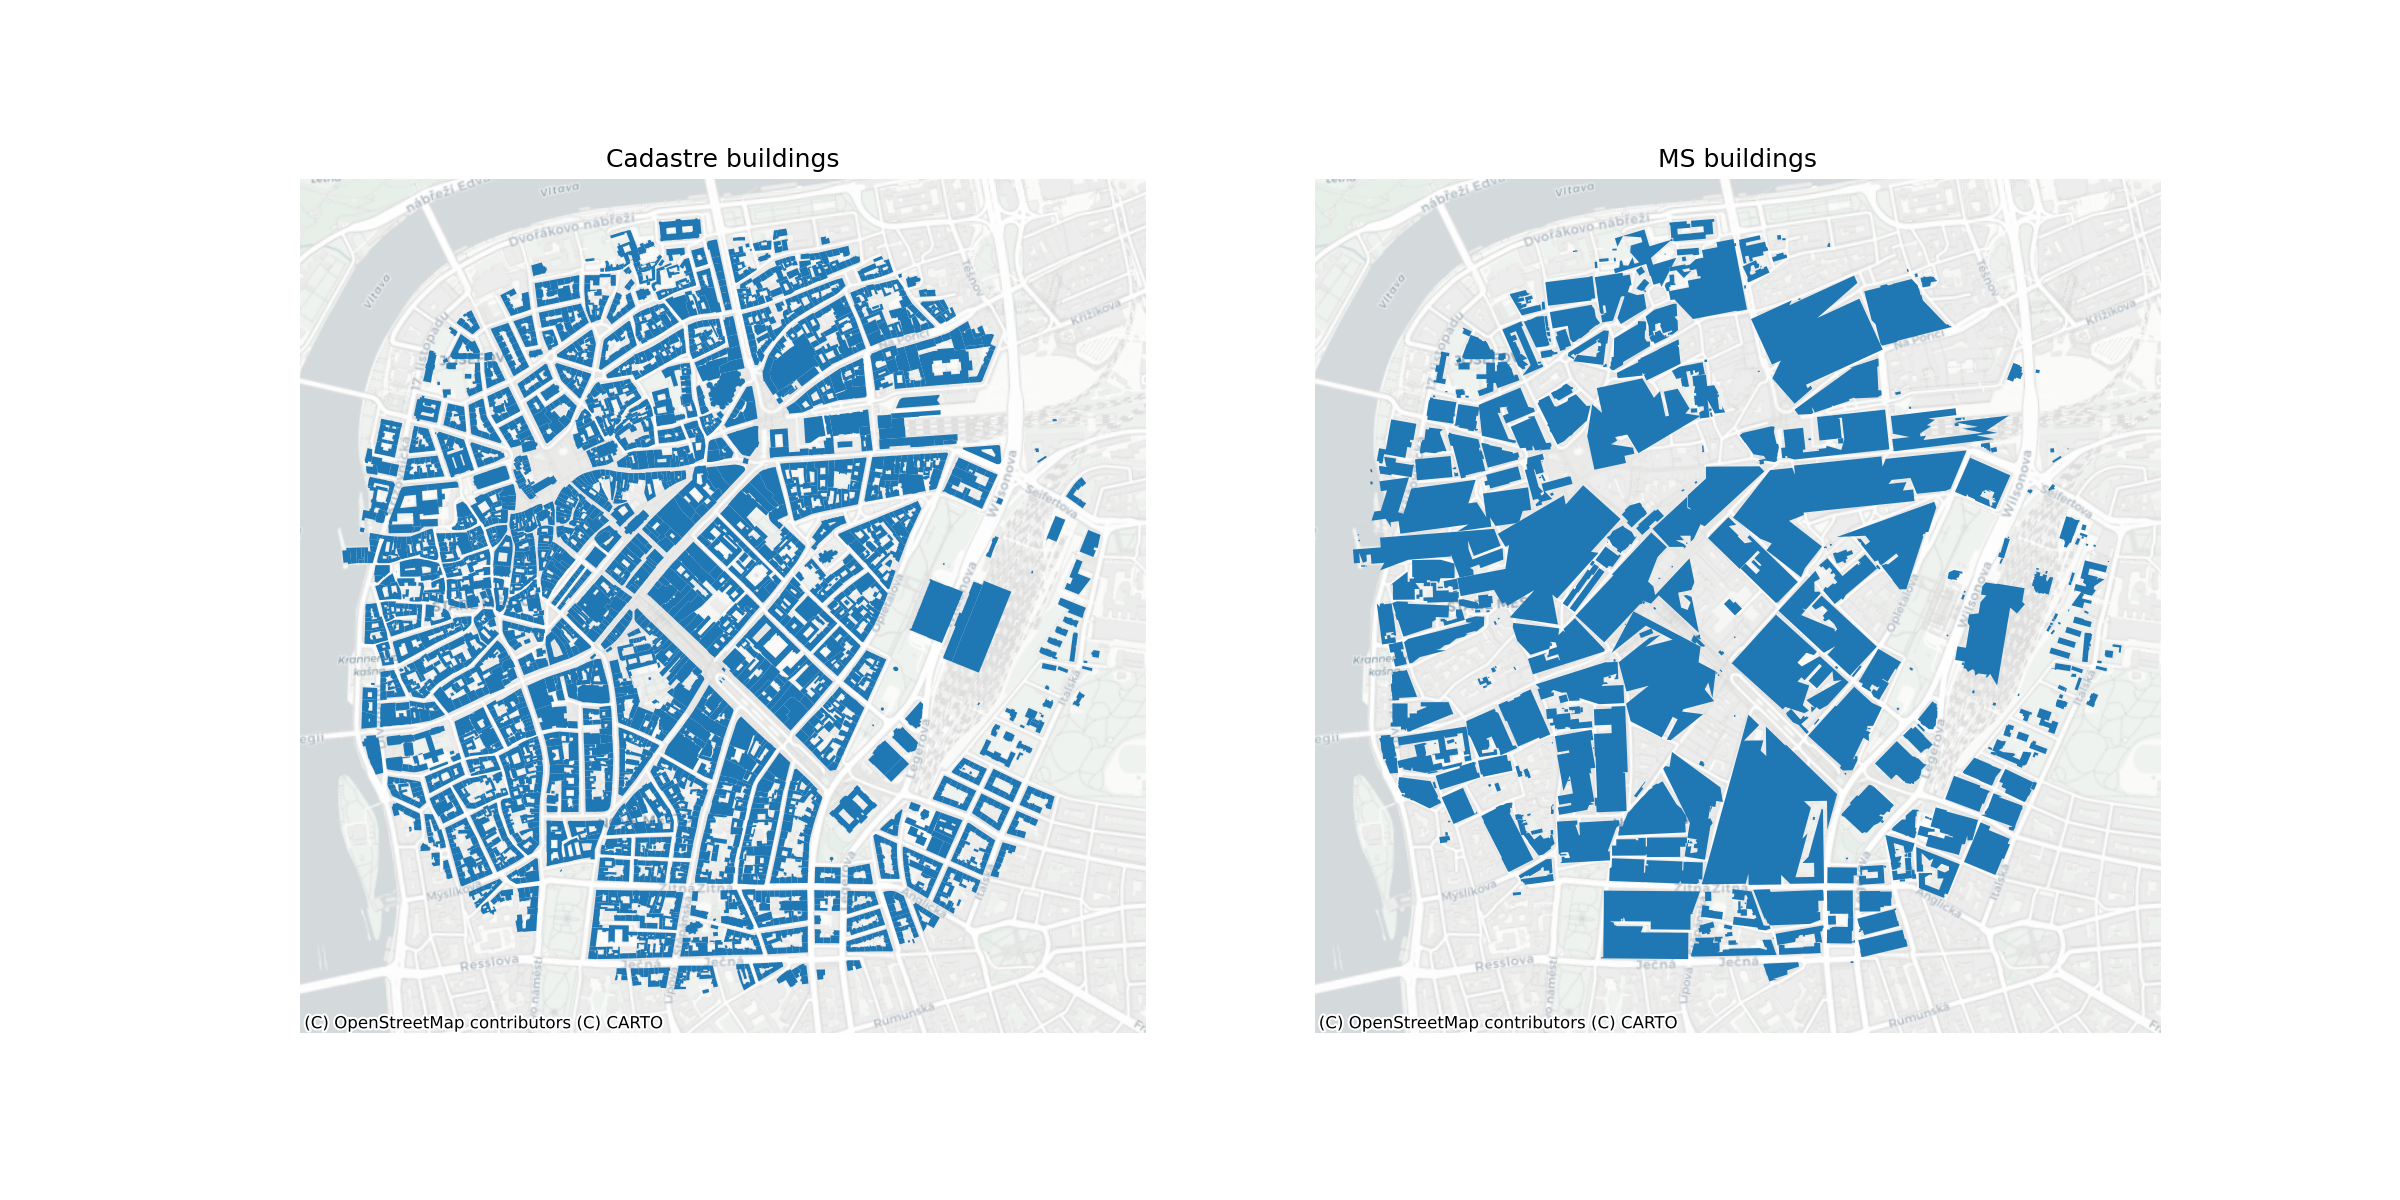
\includegraphics[width=\linewidth,height=4.16667in,keepaspectratio]{../figures/algo_design/building_comparison.png}

}

\caption{Comparison between MS buildings and cadastre level buildings in
central Prague}

\end{figure}%

Before dealing with any morphological assessment, the polygons need to
undergo basic topological preprocessing.

The first step in the building data processing is to split up
multi-polygons and make the geometries valid. The second step, is to
simplify the polygons in order to accurately represent the corners of
buildings and other shape related characteristics. Next, to filter out
any buildings that have an area larger than 200,000 sq.m. This is done
since some artefacts such as construction sites, mines or tunnels might
be included in the data as buildings. The next step is to merge
overlapping buildings that either: overlap for at least 10 percent of
their areas, or one of them has less than 50 sq.m. in total area. This
is done to merge buildings and building parts, since cadastre
definitions of these two polygon types are inconsistent and sometimes
buildings are assigned as building parts or vice versa. This step merges
the buildings and its parts into one polygon. Finally, the preprocessing
pipeline snaps nearby buildings together and fills gaps in the polygons
that are less than 10 square cm. These two steps aim to address some
common topological issues, such as missing slivers with almost zero
areas between multiple or inside individual building polygons.
Nevertheless, even after the preprocessing numerous topological issues
remain and therefore we take this into account in subsequent analysis
steps.

\paragraph{Overture Streets}\label{overture-streets}

The street network is a direct download from Overture Maps
Transportation theme, a processed subset of data from OpenStreetMap,
which has global coverage and high quality data. Since the dataset
includes multiple segments types, including footpaths, the types of
segments used in the analysis are limited to \ldots{} . Another type of
segment that is filtered out are tunnels - the analysis strictly focuses
on two dimensions and therefore undergrounds structures adversely affect
the calculation of boundaries and characters.

The second major stage of the street processing is the simplification of
the entire street network for each subregion. The network coming from
Overture Maps, similarly to nearly any other common source, focuses on
representation of street network for transportation purposes. That means
it tends to include multiple geometries for wide boulevards where each
captures a single carriageway, complex representation of junctions or
even the smallest artefacts of transportation-based focus. However, such
a network is not directly usable for morphological analysis as it does
not capture morphological perception of street network which is usually
captured via street centrelines, omitting transportation detail. For
this reason, we apply the simplification method based on the detection
of the problematic parts of the network (Fleischmann and Vybornova 2024)
by Fleischmann, Vybornova, and Gaboardi (Forthcoming). This ensures
automatised algorithmic cleaning of street networks resulting in a
morphological representation derived from the transportation one.

\begin{figure}[H]

{\centering 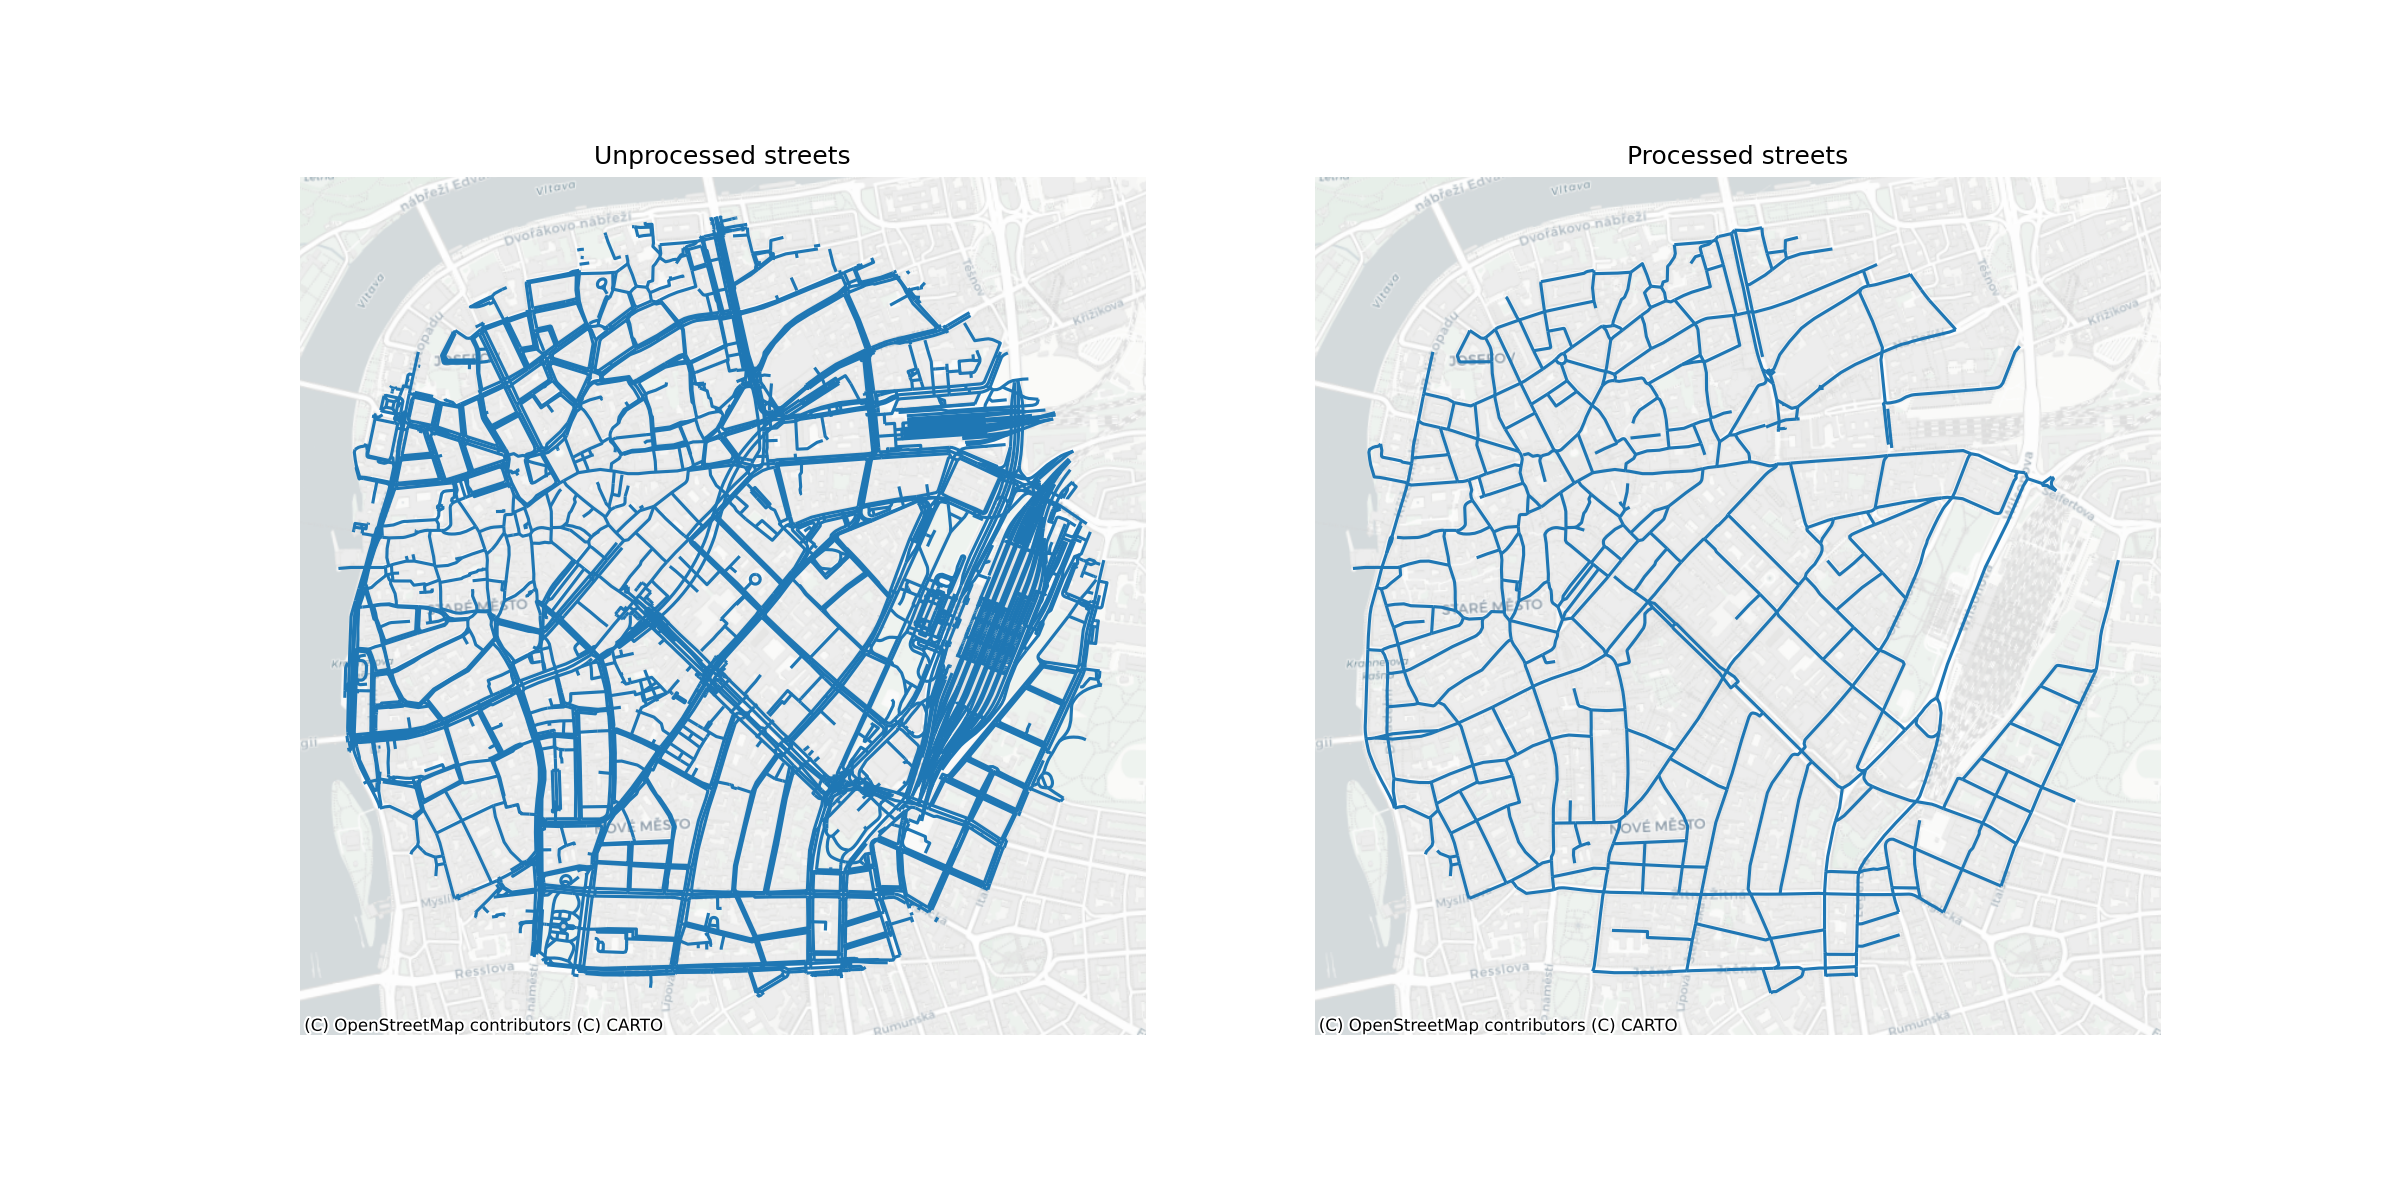
\includegraphics[width=\linewidth,height=4.16667in,keepaspectratio]{../figures/algo_design/street_processing.png}

}

\caption{Streets in central Prague}

\end{figure}%

\subsubsection{Morphometric
characterisation}\label{morphometric-characterisation}

The morphometric characterisation is directly derived from the method of
(Fleischmann and Samardzhiev Forthcoming) as closely as possible to
ensure that we minimise the conceptual differences between the
methodological backbone using the derivation of the target
classification and the the data used within our model.

\paragraph{Subregions split}\label{subregions-split}

Since the study area of interest is large and contains tens of millions
of buildings, it is divided into subregions to carry out all
computation. The separation is done based on distances between buildings
- buildings are split into subregions such that the building from one
region and its closest neighbour (another building) from another region
are at least 400 meters apart. This custom separation, rather than
official administrative divisions, ensures that all elements that may
affect morphological calculations are in the same set (subregion) and
not split across political boundaries. All processing and character
calculations are done for each region independently and in parallel.

\begin{figure}[H]

{\centering 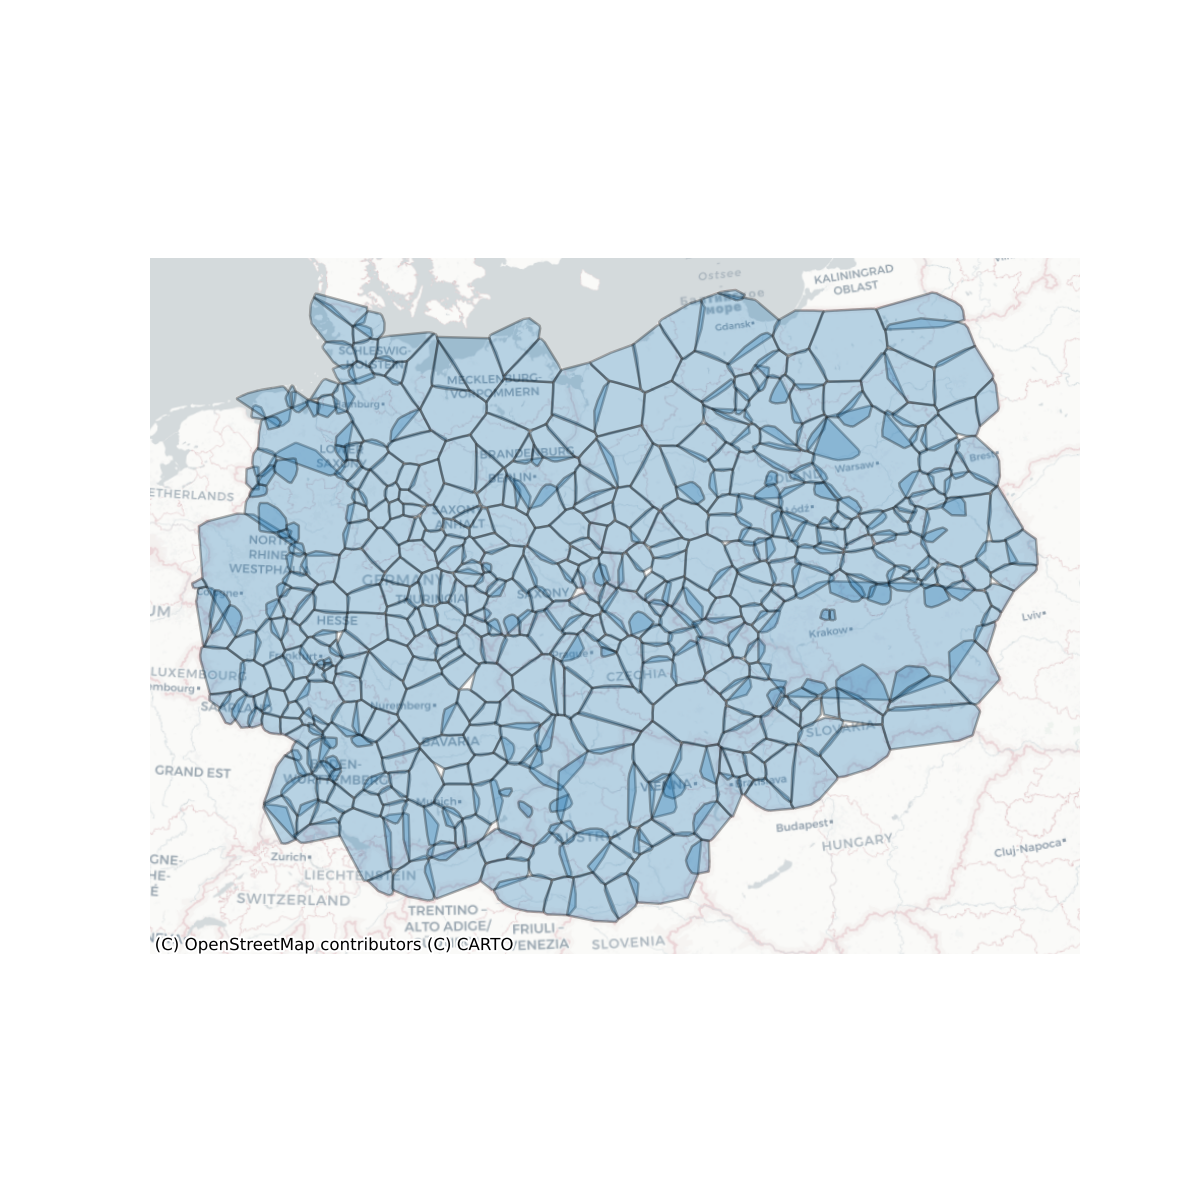
\includegraphics[width=\linewidth,height=4.16667in,keepaspectratio]{../figures/algo_design/subregions.png}

}

\caption{All subregions in the study area}

\end{figure}%

\paragraph{Elements and units}\label{elements-and-units}

There are five morphological elements used for the morphometric
characterisation - two base ones - buildings and streets and three
derived ones - enclosures, nodes, enclosed tessellation cells (ETC).
Buildings and streets are the two elements from which all other units
are derived. The core unit of analysis in the study is the enclosed
tessellation cell, which breaks down the whole study area into
small-scale units, which when taken together fully cover the area.

\subparagraph{Nodes}\label{nodes}

The first type of derived element in the study are street nodes, which
are defined as the intersection points between different streets. They
are used to calculate characteristics of the street network that capture
relationships between streets such as number of intersections, as well
as relationships between neighbouring enclosures and ETCs.

\begin{figure}[H]

{\centering 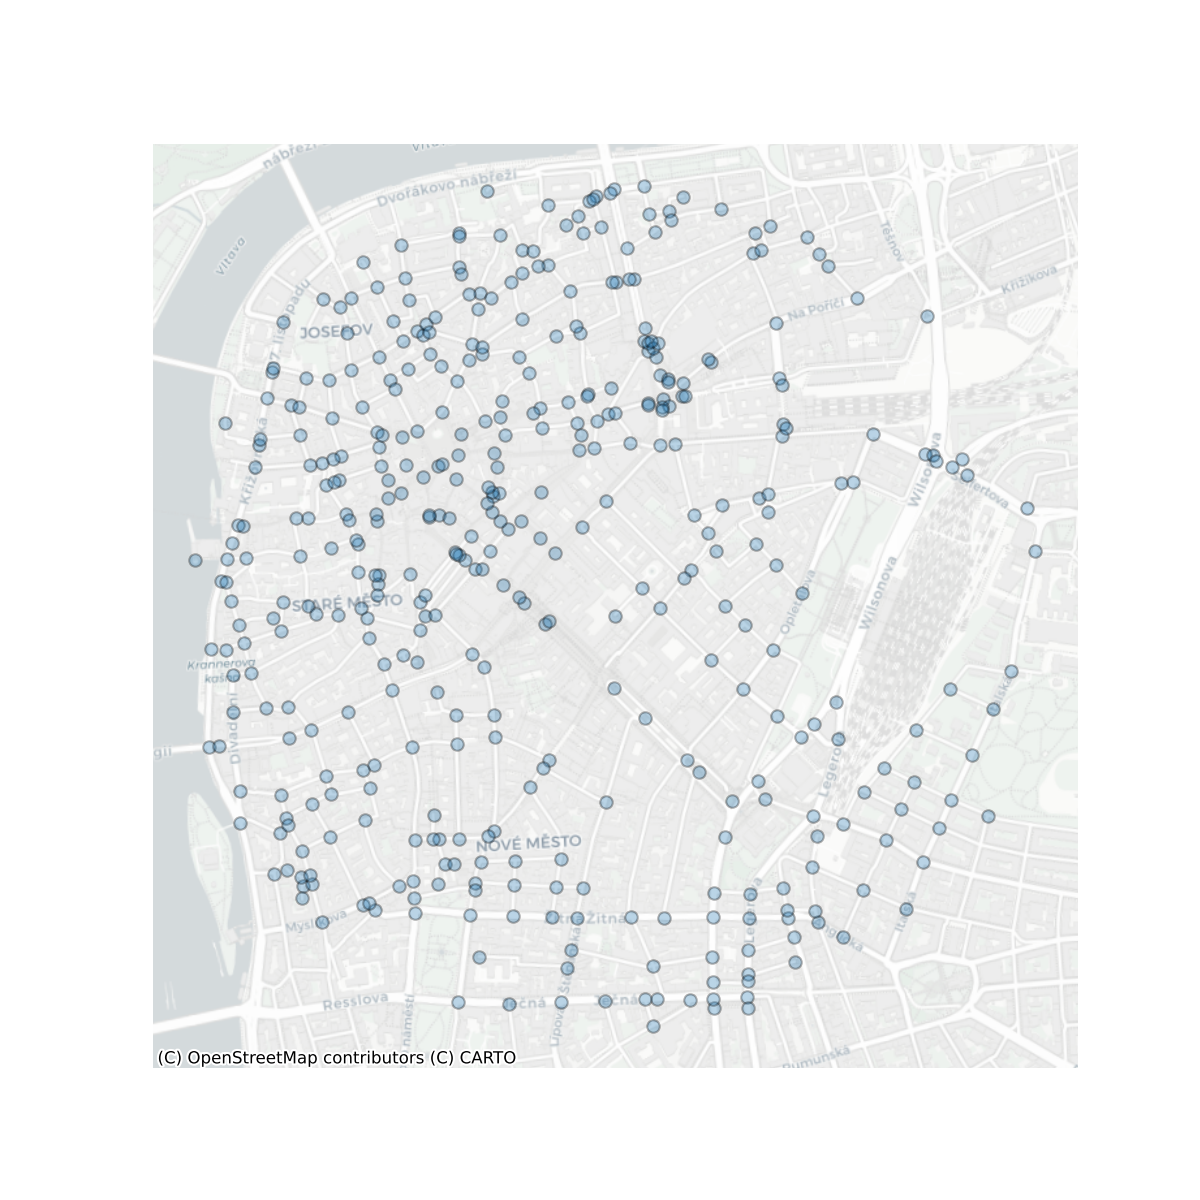
\includegraphics[width=\linewidth,height=4.16667in,keepaspectratio]{../figures/algo_design/nodes.png}

}

\caption{Nodes in central Prague}

\end{figure}%

\subparagraph{Enclosures}\label{enclosures}

Enclosures capture the characteristics of plots of land that contain
from none to (usually) multiple buildings. They are operationalised as
land delineations, surrounded by streets and other physical barriers,
which can vary in size depending on the geographic context. If an area
is in the city centre, each enclosure would approximate a single block
and multiple building units, however if it was in an industrial area it
would potentially encompass a single, or very few large buildings. In
this study, only the street network is used for barriers to minimise the
data dependency. Furthermore, enclosures are used to delineate the
boundaries of enclosed tessellation cells to the surrounding streets -
i.e.~representing physical barriers.

In this study, enclosure delineation is further modified by introducing
a variable, individual bandwidth for every building, as opposed to the
global one used by (Fleischmann et al. 2022) or none using in generic
enclosure delineation. This is done to limit the boundaries effects
around the edges of cities and towns - i.e.~cells on the edges of cities
in (Fleischmann et al. 2022) are always large because there are no
surrounding buildings and their cells resemble those of large buildings
with lots of empty space around them. The limits used here are
calculated through a Gabriel graph-based filtration of the subregion,
which takes into account the surrounding neighbours structure around
every ETC. For example, in row housing the buffer will be relatively
small, in single family housing estates the buffer will be larger, and
in industrial areas larger still; regardless of whether or not these
buildings are in the middle of cities or around their edges. The
detailed technical implementation is out of scope of this Technical
Note.

\begin{figure}[H]

{\centering 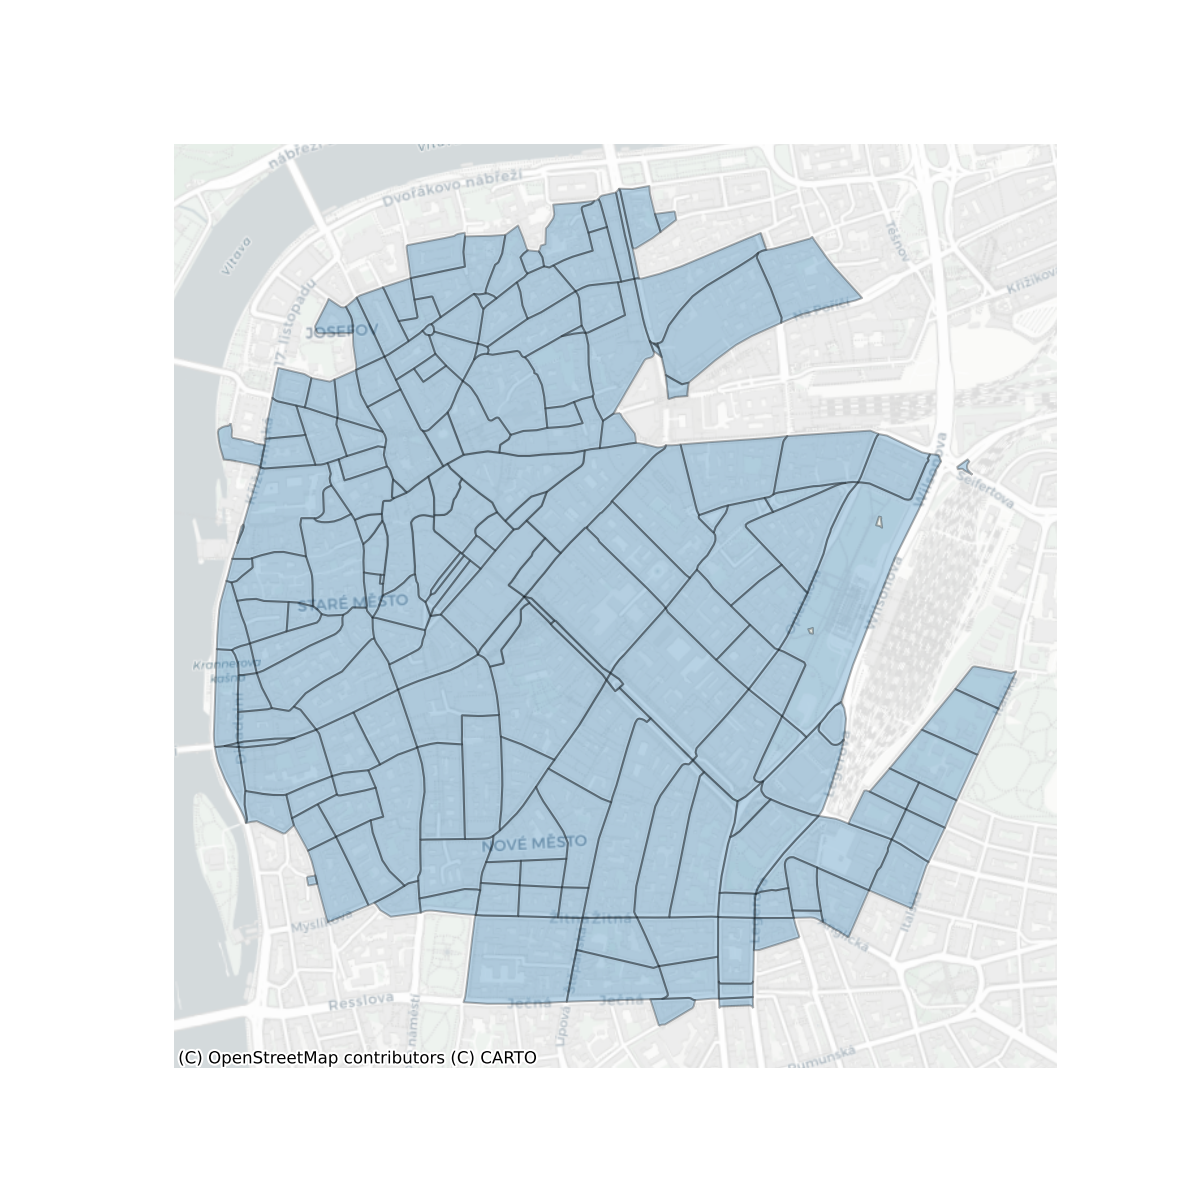
\includegraphics[width=\linewidth,height=4.16667in,keepaspectratio]{../figures/algo_design/enclosures.png}

}

\caption{Enclosures in central Prague}

\end{figure}%

\subparagraph{Enclosed Tessellation
Cells}\label{enclosed-tessellation-cells}

Enclosed Tessellation Cells are the core unit used for the analysis and
the one used to combine aspects of all of the other four elements. To
operationalise it, the study follows the definition by (Fleischmann et
al. 2022) - ``the portion of space that results from growing a
morphological tessellation within an enclosure delineated by a series of
natural or built barriers identified from the literature on urban form,
function and perception'', where the morphological tessellation is a
delineation of the space based on Voronoi polygons centred around
buildings. The boundaries of ETCs also represent the closest area of
land to each building, than to any other building within an enclosure.
Because of this feature, ETCs intersect with all other elements and are
the unit that links together the characteristics of the four other
elements. In some cases, if there are no buildings within the enclosure
the whole enclosure is treated as an `empty' tessellation cell.

\begin{figure}[H]

{\centering 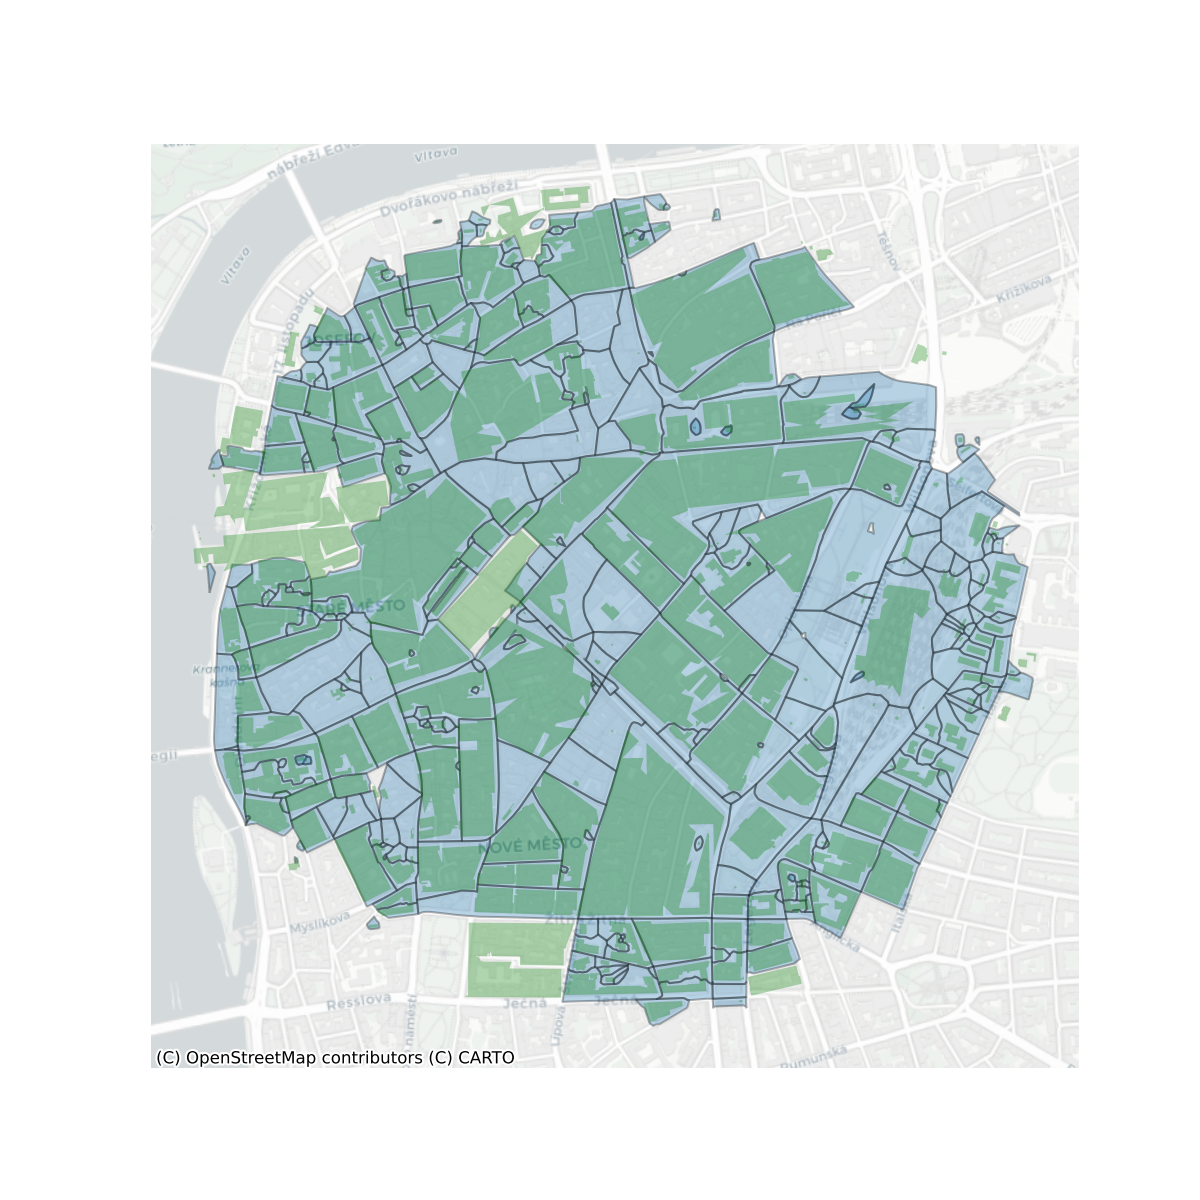
\includegraphics[width=\linewidth,height=4.16667in,keepaspectratio]{../figures/algo_design/tessellations.png}

}

\caption{Enclosed tessellation cells in central Prague}

\end{figure}%

\subparagraph{Morphometric Characters}\label{morphometric-characters}

Characteristics describing the interactions of these elements, and the
elements themselves are calculated at three scales: small - covering
only aspects of the element; medium - covering aspects of the element
and neighbouring elements and large - covering neighbouring elements up
to five topological neighbours. In total there are 52 morphometric
characters calculated described in the list below, which come directly
from the list of characters used to derive the target classification.

\begin{enumerate}
\def\labelenumi{\arabic{enumi}.}
\tightlist
\item
  \textbf{Area of a building} is denoted as
\end{enumerate}

\begin{enumerate}
\def\labelenumi{(\arabic{enumi})}
\tightlist
\item
  \(a_{blg}\)
\end{enumerate}

and defined as an area covered by a building footprint in
m\textsuperscript{2} .

\begin{enumerate}
\def\labelenumi{\arabic{enumi}.}
\setcounter{enumi}{1}
\tightlist
\item
  \textbf{Perimeter of a building} is denoted as
\end{enumerate}

\begin{enumerate}
\def\labelenumi{(\arabic{enumi})}
\setcounter{enumi}{1}
\tightlist
\item
  \(p_{blg}\)
\end{enumerate}

and defined as the sum of lengths of the building exterior walls in m.

\begin{enumerate}
\def\labelenumi{\arabic{enumi}.}
\setcounter{enumi}{2}
\tightlist
\item
  \textbf{Courtyard area of a building} is denoted as
\end{enumerate}

\begin{enumerate}
\def\labelenumi{(\arabic{enumi})}
\setcounter{enumi}{2}
\tightlist
\item
  \(a_{blg_c}\)
\end{enumerate}

and defined as the sum of areas of interior holes in footprint polygons
in m\textsuperscript{2}.

\begin{enumerate}
\def\labelenumi{\arabic{enumi}.}
\setcounter{enumi}{3}
\tightlist
\item
  \textbf{Circular compactness of a building} is denoted as
\end{enumerate}

\begin{enumerate}
\def\labelenumi{(\arabic{enumi})}
\setcounter{enumi}{3}
\tightlist
\item
  \(CCo_{blg} = \frac{a_{blg}}{a_{blgC}}\)
\end{enumerate}

where \(a_{blgC}\) is an area of minimal enclosing circle. It captures
the relation of building footprint shape to its minimal enclosing
circle, illustrating the similarity of shape and circle (Dibble et al.
2015).

\begin{enumerate}
\def\labelenumi{\arabic{enumi}.}
\setcounter{enumi}{4}
\tightlist
\item
  \textbf{Corners of a building} is denoted as
\end{enumerate}

\begin{enumerate}
\def\labelenumi{(\arabic{enumi})}
\setcounter{enumi}{4}
\tightlist
\item
  \(Cor_{blg} = \sum_{i=1}^{n}{c_{blg}}\)
\end{enumerate}

where \(c_{blg}\) is defined as a vertex of building exterior shape with
an angle between adjacent line segments \(\leq\) 170 degrees. It uses
only external shape (\texttt{shapely.geometry.exterior}), courtyards are
not included. Character is adapted from (Steiniger et al. 2008) to
exclude non-corner-like vertices.

\begin{enumerate}
\def\labelenumi{\arabic{enumi}.}
\setcounter{enumi}{5}
\tightlist
\item
  \textbf{Squareness of a building} is denoted as
\end{enumerate}

\begin{enumerate}
\def\labelenumi{(\arabic{enumi})}
\setcounter{enumi}{5}
\tightlist
\item
  \(Squ_{blg} =  \frac{\sum_{i=1}^{n} D_{c_{blg_i}}}{n}\)
\end{enumerate}

where \(D\) is the deviation of angle of corner \(c_{blg_i}\) from 90
degrees and \(n\) is a number of corners.

\begin{enumerate}
\def\labelenumi{\arabic{enumi}.}
\setcounter{enumi}{6}
\tightlist
\item
  \textbf{Equivalent rectangular index of a building} is denoted as
\end{enumerate}

\begin{enumerate}
\def\labelenumi{(\arabic{enumi})}
\setcounter{enumi}{6}
\tightlist
\item
  \(ERI_{blg} =  \sqrt{{a_{blg}} \over {a_{blgB}}} * {p_{blgB} \over p_{blg}}\)
\end{enumerate}

where \(a_{blgB}\) is an area of a minimal rotated bounding rectangle of
a building (MBR) footprint and \(p_{blgB}\) its perimeter of MBR. It is
a measure of shape complexity identified by Basaraner and Cetinkaya
(2017) as the shape characters with the best performance.

\begin{enumerate}
\def\labelenumi{\arabic{enumi}.}
\setcounter{enumi}{7}
\tightlist
\item
  \textbf{Elongation of a building} is denoted as
\end{enumerate}

\begin{enumerate}
\def\labelenumi{(\arabic{enumi})}
\setcounter{enumi}{7}
\tightlist
\item
  \(Elo_{blg} =  \frac{l_{blgB}}{w_{blgB}}\)
\end{enumerate}

where \(l_{blgB}\) is length of MBR and \(w_{blgB}\) is width of MBR. It
captures the ratio of shorter to the longer dimension of MBR to
indirectly capture the deviation of the shape from a square (Schirmer
and Axhausen 2015).

\begin{enumerate}
\def\labelenumi{\arabic{enumi}.}
\setcounter{enumi}{8}
\tightlist
\item
  \textbf{Centroid - corner distance deviation of a building} is denoted
  as
\end{enumerate}

\begin{enumerate}
\def\labelenumi{(\arabic{enumi})}
\setcounter{enumi}{8}
\tightlist
\item
  \(CCD_{blg} =  \sqrt{\frac{1}{n} \sum_{i=1}^{n}\left(ccd_{i}-\bar{ccd}\right)^{2}}\)
\end{enumerate}

where \(ccd_i\) is a distance between centroid and corner \(i\) and
\(\bar{ccd}\) is mean of all distances. It captures a variety of shape.
As a corner is considered vertex with angle \textless{} 170º to reflect
potential circularity of object and topological imprecision of building
polygon.

\begin{enumerate}
\def\labelenumi{\arabic{enumi}.}
\setcounter{enumi}{9}
\tightlist
\item
  \textbf{Centroid - corner mean distance of a building} is denoted as
\end{enumerate}

\begin{enumerate}
\def\labelenumi{(\arabic{enumi})}
\setcounter{enumi}{9}
\tightlist
\item
  \(CCM_{blg} =\frac{1}{n}\left(\sum_{i=1}^{n} ccd_{i}\right)\)
\end{enumerate}

where \(ccd_i\) is a distance between centroid and corner \(i\). It is a
character measuring a dimension of the object dependent on its shape
(Schirmer and Axhausen 2015).

\begin{enumerate}
\def\labelenumi{\arabic{enumi}.}
\setcounter{enumi}{10}
\tightlist
\item
  \textbf{Longest axis length of a tessellation cell} is denoted as
\end{enumerate}

\begin{enumerate}
\def\labelenumi{(\arabic{enumi})}
\setcounter{enumi}{10}
\tightlist
\item
  \(LAL_{cell} = d_{cellC}\)
\end{enumerate}

where \(d_{cellC}\) is a diameter of the minimal circumscribed circle
around the tessellation cell polygon. The axis itself does not have to
be fully within the polygon. It could be seen as a proxy of plot depth
for tessellation-based analysis.

\begin{enumerate}
\def\labelenumi{\arabic{enumi}.}
\setcounter{enumi}{11}
\tightlist
\item
  \textbf{Area of a tessellation cell} is denoted as
\end{enumerate}

\begin{enumerate}
\def\labelenumi{(\arabic{enumi})}
\setcounter{enumi}{11}
\tightlist
\item
  \(a_{cell}\)
\end{enumerate}

and defined as an area covered by a tessellation cell footprint in
m\textsuperscript{2}.

\begin{enumerate}
\def\labelenumi{\arabic{enumi}.}
\setcounter{enumi}{12}
\tightlist
\item
  \textbf{Circular compactness of a tessellation cell} is denoted as
\end{enumerate}

\begin{enumerate}
\def\labelenumi{(\arabic{enumi})}
\setcounter{enumi}{12}
\tightlist
\item
  \(CCo_{cell} = \frac{a_{cell}}{a_{cellC}}\)
\end{enumerate}

where \(a_{cellC}\) is an area of minimal enclosing circle. It captures
the relation of tessellation cell footprint shape to its minimal
enclosing circle, illustrating the similarity of shape and circle.

\begin{enumerate}
\def\labelenumi{\arabic{enumi}.}
\setcounter{enumi}{13}
\tightlist
\item
  \textbf{Equivalent rectangular index of a tessellation cell} is
  denoted as
\end{enumerate}

\begin{enumerate}
\def\labelenumi{(\arabic{enumi})}
\setcounter{enumi}{13}
\tightlist
\item
  \(ERI_{cell} =  \sqrt{{a_{cell}} \over {a_{cellB}}} * {p_{cellB} \over p_{cell}}\)
\end{enumerate}

where \(a_{cellB}\) is an area of the minimal rotated bounding rectangle
of a tessellation cell (MBR) footprint and \(p_{cellB}\) its perimeter
of MBR. It is a measure of shape complexity identified by Basaraner and
Cetinkaya (2017) as a shape character of the best performance.

\begin{enumerate}
\def\labelenumi{\arabic{enumi}.}
\setcounter{enumi}{14}
\tightlist
\item
  \textbf{Coverage area ratio of a tessellation cell} is denoted as
\end{enumerate}

\begin{enumerate}
\def\labelenumi{(\arabic{enumi})}
\setcounter{enumi}{14}
\tightlist
\item
  \(CAR_{cell} = \frac{a_{blg}}{a_{cell}}\)
\end{enumerate}

where \(a_{blg}\) is an area of a building and \(a_{cell}\) is an area
of related tessellation cell (Schirmer and Axhausen 2015). Coverage area
ratio (CAR) is one of the commonly used characters capturing
\emph{intensity} of development. However, the definitions vary based on
the spatial unit.

\begin{enumerate}
\def\labelenumi{\arabic{enumi}.}
\setcounter{enumi}{15}
\tightlist
\item
  \textbf{Floor area ratio of a tessellation cell} is denoted as
\end{enumerate}

\begin{enumerate}
\def\labelenumi{(\arabic{enumi})}
\setcounter{enumi}{15}
\tightlist
\item
  \(FAR_{cell} = \frac{fa_{blg}}{a_{cell}}\)
\end{enumerate}

where \(fa_{blg}\) is a floor area of a building and \(a_{cell}\) is an
area of related tessellation cell. Floor area could be computed based on
the number of levels or using an approximation based on building height.

\begin{enumerate}
\def\labelenumi{\arabic{enumi}.}
\setcounter{enumi}{16}
\tightlist
\item
  \textbf{Length of a street segment} is denoted as
\end{enumerate}

\begin{enumerate}
\def\labelenumi{(\arabic{enumi})}
\setcounter{enumi}{16}
\tightlist
\item
  \(l_{edg}\)
\end{enumerate}

and defined as a length of a \texttt{LineString} geometry in metres
(Dibble et al. 2015; Gil et al. 2012).

\begin{enumerate}
\def\labelenumi{\arabic{enumi}.}
\setcounter{enumi}{17}
\tightlist
\item
  \textbf{Width of a street profile} is denoted as
\end{enumerate}

\begin{enumerate}
\def\labelenumi{(\arabic{enumi})}
\setcounter{enumi}{17}
\tightlist
\item
  \(w_{sp} = \frac{1}{n}\left(\sum_{i=1}^{n} w_{i}\right)\)
\end{enumerate}

where \(w_{i}\) is width of a street section i. The algorithm generates
street sections every 3 meters alongside the street segment, and
measures mean value. In the case of the open-ended street, 50 metres is
used as a perception-based proximity limit (Araldi and Fusco 2019).

\begin{enumerate}
\def\labelenumi{\arabic{enumi}.}
\setcounter{enumi}{18}
\tightlist
\item
  \textbf{Openness of a street profile} is denoted as
\end{enumerate}

\begin{enumerate}
\def\labelenumi{(\arabic{enumi})}
\setcounter{enumi}{18}
\tightlist
\item
  \(Ope_{sp} = 1 - \frac{\sum hit}{2\sum sec}\)
\end{enumerate}

where \(\sum hit\) is a sum of section lines (left and right sides
separately) intersecting buildings and \(\sum sec\) total number of
street sections. The algorithm generates street sections every 3 meters
alongside the street segment.

\begin{enumerate}
\def\labelenumi{\arabic{enumi}.}
\setcounter{enumi}{19}
\tightlist
\item
  \textbf{Width deviation of a street profile} is denoted as
\end{enumerate}

\begin{enumerate}
\def\labelenumi{(\arabic{enumi})}
\setcounter{enumi}{19}
\tightlist
\item
  \(wDev_{sp} = \sqrt{\frac{1}{n} \sum_{i=1}^{n}\left(w_{i}-w_{sp}\right)^{2}}\)
\end{enumerate}

where \(w_{i}\) is width of a street section i and \(w_{sp}\) is mean
width. The algorithm generates street sections every 3 meters alongside
the street segment.

\begin{enumerate}
\def\labelenumi{\arabic{enumi}.}
\setcounter{enumi}{20}
\tightlist
\item
  \textbf{Linearity of a street segment} is denoted as
\end{enumerate}

\begin{enumerate}
\def\labelenumi{(\arabic{enumi})}
\setcounter{enumi}{20}
\tightlist
\item
  \(Lin_{edg} = \frac{l_{eucl}}{l_{edg}}\)
\end{enumerate}

where \(l_{eucl}\) is Euclidean distance between endpoints of a street
segment and \(l_{edg}\) is a street segment length. It captures the
deviation of a segment shape from a straight line. It is adapted from
Araldi and Fusco (2019).

\begin{enumerate}
\def\labelenumi{\arabic{enumi}.}
\setcounter{enumi}{21}
\tightlist
\item
  \textbf{Area covered by a street segment} is denoted as
\end{enumerate}

\begin{enumerate}
\def\labelenumi{(\arabic{enumi})}
\setcounter{enumi}{21}
\tightlist
\item
  \(a_{edg} = \sum_{i=1}^{n} a_{cell_i}\)
\end{enumerate}

where \(a_{cell_i}\) is an area of tessellation cell \(i\) belonging to
the street segment. It captures the area which is likely served by each
segment.

\begin{enumerate}
\def\labelenumi{\arabic{enumi}.}
\setcounter{enumi}{22}
\tightlist
\item
  \textbf{Buildings per meter of a street segment} is denoted as
\end{enumerate}

\begin{enumerate}
\def\labelenumi{(\arabic{enumi})}
\setcounter{enumi}{22}
\tightlist
\item
  \(BpM_{edg} = \frac{\sum blg}{l_{edg}}\)
\end{enumerate}

where \(\sum blg\) is a number of buildings belonging to a street
segment and \(l_{edg}\) is a length of a street segment. It reflects the
granularity of development along each segment.

\begin{enumerate}
\def\labelenumi{\arabic{enumi}.}
\setcounter{enumi}{23}
\tightlist
\item
  \textbf{Area covered by a street node} is denoted as
\end{enumerate}

\begin{enumerate}
\def\labelenumi{(\arabic{enumi})}
\setcounter{enumi}{23}
\tightlist
\item
  \(a_{node} = \sum_{i=1}^{n} a_{cell_i}\)
\end{enumerate}

where \(a_{cell_i}\) is an area of tessellation cell \(i\) belonging to
the street node. It captures the area which is likely served by each
node.

\begin{enumerate}
\def\labelenumi{\arabic{enumi}.}
\setcounter{enumi}{24}
\tightlist
\item
  \textbf{Shared walls ratio of adjacent buildings} is denoted as
\end{enumerate}

\begin{enumerate}
\def\labelenumi{(\arabic{enumi})}
\setcounter{enumi}{24}
\tightlist
\item
  \(SWR_{blg} = \frac{p_{blg_{shared}}}{p_{blg}}\)
\end{enumerate}

where \(p_{blg_{shared}}\) is a length of a perimeter shared with
adjacent buildings and \(p_{blg}\) is a perimeter of a building. It
captures the amount of wall space facing the open space (Hamaina, Leduc,
and Moreau 2012).

\begin{enumerate}
\def\labelenumi{\arabic{enumi}.}
\setcounter{enumi}{25}
\tightlist
\item
  \textbf{‌Mean distance to neighbouring buildings} is denoted as
\end{enumerate}

\begin{enumerate}
\def\labelenumi{(\arabic{enumi})}
\setcounter{enumi}{25}
\tightlist
\item
  \(NDi_{blg} = \frac{1}{n} \sum_{i=1}^{n} d_{blg, blg_i}\)
\end{enumerate}

where \(d_{blg, blg_i}\) is a distance between building and building
\(i\) on a neighbouring tessellation cell. It is adapted from Hijazi et
al. (2016). It captures the average proximity to other buildings.

\begin{enumerate}
\def\labelenumi{\arabic{enumi}.}
\setcounter{enumi}{26}
\tightlist
\item
  \textbf{Weighted neighbours of a tessellation cell} is denoted as
\end{enumerate}

\begin{enumerate}
\def\labelenumi{(\arabic{enumi})}
\setcounter{enumi}{26}
\tightlist
\item
  \(WNe_{cell} = \frac{\sum cell_n}{p_{cell}}\)
\end{enumerate}

where \(\sum cell_n\) is a number of cell neighbours and \(p_{cell}\) is
a perimeter of a cell. It reflects granularity of morphological
tessellation.

\begin{enumerate}
\def\labelenumi{\arabic{enumi}.}
\setcounter{enumi}{27}
\tightlist
\item
  \textbf{Area covered by neighbouring cells} is denoted as
\end{enumerate}

\begin{enumerate}
\def\labelenumi{(\arabic{enumi})}
\setcounter{enumi}{27}
\tightlist
\item
  \(a_{cell_n} = \sum_{i=1}^{n} a_{cell_i}\)
\end{enumerate}

where \(a_{cell_i}\) is area of tessellation cell \(i\) within
topological distance 1. It captures the scale of morphological
tessellation.

\begin{enumerate}
\def\labelenumi{\arabic{enumi}.}
\setcounter{enumi}{28}
\tightlist
\item
  \textbf{Reached cells by neighbouring segments} is denoted as
\end{enumerate}

\begin{enumerate}
\def\labelenumi{(\arabic{enumi})}
\setcounter{enumi}{28}
\tightlist
\item
  \(RC_{edg_n} = \sum_{i=1}^{n} cells_{edg_i}\)
\end{enumerate}

where \(cells_{edg_i}\) is number of tessellation cells on segment \(i\)
within topological distance 1. It captures accessible granularity.

\begin{enumerate}
\def\labelenumi{\arabic{enumi}.}
\setcounter{enumi}{29}
\tightlist
\item
  \textbf{Reached area by neighbouring segments} is denoted as
\end{enumerate}

\begin{enumerate}
\def\labelenumi{(\arabic{enumi})}
\setcounter{enumi}{29}
\tightlist
\item
  \(a_{edg_n} = \sum_{i=1}^{n} a_{edg_i}\)
\end{enumerate}

where \(a_{edg_i}\) is an area covered by a street segment \(i\) within
topological distance 1. It captures an accessible area.

\begin{enumerate}
\def\labelenumi{\arabic{enumi}.}
\setcounter{enumi}{30}
\tightlist
\item
  \textbf{Degree of a street node} is denoted as
\end{enumerate}

\begin{enumerate}
\def\labelenumi{(\arabic{enumi})}
\setcounter{enumi}{30}
\tightlist
\item
  \(deg_{node_i} = \sum_{j} edg_{i j}\)
\end{enumerate}

where \(edg_{i j}\) is an edge of a street network between node \(i\)
and node \(j\). It reflects the basic degree centrality.

\begin{enumerate}
\def\labelenumi{\arabic{enumi}.}
\setcounter{enumi}{31}
\tightlist
\item
  \textbf{Mean distance to neighbouring nodes from a street node} is
  denoted as
\end{enumerate}

\begin{enumerate}
\def\labelenumi{(\arabic{enumi})}
\setcounter{enumi}{31}
\tightlist
\item
  \(MDi_{node} = \frac{1}{n} \sum_{i=1}^{n} d_{node, node_i}\)
\end{enumerate}

where \(d_{node, node_i}\) is a distance between node and node \(i\)
within topological distance 1. It captures the average proximity to
other nodes.

\begin{enumerate}
\def\labelenumi{\arabic{enumi}.}
\setcounter{enumi}{32}
\tightlist
\item
  \textbf{Reached cells by neighbouring nodes} is denoted as
\end{enumerate}

\begin{enumerate}
\def\labelenumi{(\arabic{enumi})}
\setcounter{enumi}{32}
\tightlist
\item
  \(RC_{node_n} = \sum_{i=1}^{n} cells_{node_i}\)
\end{enumerate}

where \(cells_{node_i}\) is number of tessellation cells on node \(i\)
within topological distance 1. It captures accessible granularity.

\begin{enumerate}
\def\labelenumi{\arabic{enumi}.}
\setcounter{enumi}{33}
\tightlist
\item
  \textbf{Reached area by neighbouring nodes} is denoted as
\end{enumerate}

\begin{enumerate}
\def\labelenumi{(\arabic{enumi})}
\setcounter{enumi}{33}
\tightlist
\item
  \(a_{node_n} = \sum_{i=1}^{n} a_{node_i}\)
\end{enumerate}

where \(a_{node_i}\) is an area covered by a street node \(i\) within
topological distance 1. It captures an accessible area.

\begin{enumerate}
\def\labelenumi{\arabic{enumi}.}
\setcounter{enumi}{34}
\tightlist
\item
  \textbf{Number of courtyards of adjacent buildings} is denoted as
\end{enumerate}

\begin{enumerate}
\def\labelenumi{(\arabic{enumi})}
\setcounter{enumi}{34}
\tightlist
\item
  \(NCo_{blg_{adj}}\)
\end{enumerate}

where \(NCo_{blg_{adj}}\) is a number of interior rings of a polygon
composed of footprints of adjacent buildings (Schirmer and Axhausen
2015).

\begin{enumerate}
\def\labelenumi{\arabic{enumi}.}
\setcounter{enumi}{35}
\tightlist
\item
  \textbf{Perimeter wall length of adjacent buildings} is denoted as
\end{enumerate}

\begin{enumerate}
\def\labelenumi{(\arabic{enumi})}
\setcounter{enumi}{35}
\tightlist
\item
  \(p_{blg_{adj}}\)
\end{enumerate}

where \(p_{blg_{adj}}\) is a length of an exterior ring of a polygon
composed of footprints of adjacent buildings.

\begin{enumerate}
\def\labelenumi{\arabic{enumi}.}
\setcounter{enumi}{36}
\tightlist
\item
  \textbf{Mean inter-building distance between neighbouring buildings}
  is denoted as
\end{enumerate}

\begin{enumerate}
\def\labelenumi{(\arabic{enumi})}
\setcounter{enumi}{36}
\tightlist
\item
  \(IBD_{blg} = \frac{1}{n} \sum_{i=1}^{n} d_{blg, blg_i}\)
\end{enumerate}

where \(d_{blg, blg_i}\) is a distance between building and building
\(i\) on a tessellation cell within topological distance 3. It is
adapted from Caruso, Hilal, and Thomas (2017). It captures the average
proximity between buildings.

\begin{enumerate}
\def\labelenumi{\arabic{enumi}.}
\setcounter{enumi}{37}
\tightlist
\item
  \textbf{‌Building adjacency of neighbouring buildings} is denoted as
\end{enumerate}

\begin{enumerate}
\def\labelenumi{(\arabic{enumi})}
\setcounter{enumi}{37}
\tightlist
\item
  \(BuA_{blg} = \frac{\sum blg_{adj}}{\sum blg}\)
\end{enumerate}

where \(\sum blg_{adj}\) is a number of joined built-up structures
within topological distance three and \(\sum blg\) is a number of
buildings within topological distance 3. It is adapted from Vanderhaegen
and Canters (2017).

\begin{enumerate}
\def\labelenumi{\arabic{enumi}.}
\setcounter{enumi}{38}
\tightlist
\item
  \textbf{Weighted reached blocks of neighbouring tessellation cells} is
  denoted as
\end{enumerate}

\begin{enumerate}
\def\labelenumi{(\arabic{enumi})}
\setcounter{enumi}{38}
\tightlist
\item
  \(WRB_{cell} = \frac{\sum blk}{\sum_{i=1}^{n} a_{cell_i}}\)
\end{enumerate}

where \(\sum blk\) is a number of blocks within topological distance
three and \(a_{cell_i}\) is an area of tessellation cell \(i\) within
topological distance three.

\begin{enumerate}
\def\labelenumi{\arabic{enumi}.}
\setcounter{enumi}{39}
\tightlist
\item
  \textbf{Local meshedness of a street network} is denoted as
\end{enumerate}

\begin{enumerate}
\def\labelenumi{(\arabic{enumi})}
\setcounter{enumi}{39}
\tightlist
\item
  \(Mes_{node}= \frac{e-v+1}{2 v-5}\)
\end{enumerate}

where \(e\) is a number of edges in a subgraph, and \(v\) is the number
of nodes in a subgraph (Feliciotti 2018). A subgraph is defined as a
network within topological distance five around a node.

\begin{enumerate}
\def\labelenumi{\arabic{enumi}.}
\setcounter{enumi}{40}
\tightlist
\item
  \textbf{Mean segment length of a street network} is denoted as
\end{enumerate}

\begin{enumerate}
\def\labelenumi{(\arabic{enumi})}
\setcounter{enumi}{40}
\tightlist
\item
  \(MSL_{edg} = \frac{1}{n} \sum_{i=1}^{n} l_{edg_i}\)
\end{enumerate}

where \(l_{edg_i}\) is a length of a street segment \(i\) within a
topological distance 3 around a segment.

\begin{enumerate}
\def\labelenumi{\arabic{enumi}.}
\setcounter{enumi}{41}
\tightlist
\item
  \textbf{Cul-de-sac length of a street network} is denoted as
\end{enumerate}

\begin{enumerate}
\def\labelenumi{(\arabic{enumi})}
\setcounter{enumi}{41}
\tightlist
\item
  \(CDL_{node} = \sum_{i=1}^{n} l_{edg_i}, \text { if }edg_i \text { is cul-de-sac}\)
\end{enumerate}

where \(l_{edg_i}\) is a length of a street segment \(i\) within a
topological distance 3 around a node.

\begin{enumerate}
\def\labelenumi{\arabic{enumi}.}
\setcounter{enumi}{42}
\tightlist
\item
  \textbf{Reached cells by street network segments} is denoted as
\end{enumerate}

\begin{enumerate}
\def\labelenumi{(\arabic{enumi})}
\setcounter{enumi}{42}
\tightlist
\item
  \(RC_{edg} = \sum_{i=1}^{n} cells_{edg_i}\)
\end{enumerate}

where \(cells_{edg_i}\) is number of tessellation cells on segment \(i\)
within topological distance 3. It captures accessible granularity.

\begin{enumerate}
\def\labelenumi{\arabic{enumi}.}
\setcounter{enumi}{43}
\tightlist
\item
  \textbf{Node density of a street network} is denoted as
\end{enumerate}

\begin{enumerate}
\def\labelenumi{(\arabic{enumi})}
\setcounter{enumi}{43}
\tightlist
\item
  \(D_{node} = \frac{\sum node}{\sum_{i=1}^{n} l_{edg_i}}\)
\end{enumerate}

where \(\sum node\) is a number of nodes within a subgraph and
\(l_{edg_i}\) is a length of a segment \(i\) within a subgraph. A
subgraph is defined as a network within topological distance five around
a node.

\begin{enumerate}
\def\labelenumi{\arabic{enumi}.}
\setcounter{enumi}{44}
\tightlist
\item
  \textbf{Reached cells by street network nodes} is denoted as
\end{enumerate}

\begin{enumerate}
\def\labelenumi{(\arabic{enumi})}
\setcounter{enumi}{44}
\tightlist
\item
  \(RC_{node_{net}} = \sum_{i=1}^{n} cells_{node_i}\)
\end{enumerate}

where \(cells_{node_i}\) is number of tessellation cells on node \(i\)
within topological distance 3. It captures accessible granularity.

\begin{enumerate}
\def\labelenumi{\arabic{enumi}.}
\setcounter{enumi}{45}
\tightlist
\item
  \textbf{Reached area by street network nodes} is denoted as
\end{enumerate}

\begin{enumerate}
\def\labelenumi{(\arabic{enumi})}
\setcounter{enumi}{45}
\tightlist
\item
  \(a_{node_{net}} = \sum_{i=1}^{n} a_{node_i}\)
\end{enumerate}

where \(a_{node_i}\) is an area covered by a street node \(i\) within
topological distance 3. It captures an accessible area.

\begin{enumerate}
\def\labelenumi{\arabic{enumi}.}
\setcounter{enumi}{46}
\tightlist
\item
  \textbf{Proportion of cul-de-sacs within a street network} is denoted
  as
\end{enumerate}

\begin{enumerate}
\def\labelenumi{(\arabic{enumi})}
\setcounter{enumi}{46}
\tightlist
\item
  \(pCD_{node} = \frac{\sum_{i=1}^{n} node_i, \text { if }deg_{node_i} = 1}{\sum_{i=1}^{n} node_i}\)
\end{enumerate}

where \(node_i\) is a node whiting topological distance five around a
node. Adapted from (Boeing 2017).

\begin{enumerate}
\def\labelenumi{\arabic{enumi}.}
\setcounter{enumi}{47}
\tightlist
\item
  \textbf{Proportion of 3-way intersections within a street network} is
  denoted as
\end{enumerate}

\begin{enumerate}
\def\labelenumi{(\arabic{enumi})}
\setcounter{enumi}{47}
\tightlist
\item
  \(p3W_{node} = \frac{\sum_{i=1}^{n} node_i, \text { if }deg_{node_i} = 3}{\sum_{i=1}^{n} node_i}\)
\end{enumerate}

where \(node_i\) is a node whiting topological distance five around a
node. Adapted from (Boeing 2017).

\begin{enumerate}
\def\labelenumi{\arabic{enumi}.}
\setcounter{enumi}{48}
\tightlist
\item
  \textbf{Proportion of 4-way intersections within a street network} is
  denoted as
\end{enumerate}

\begin{enumerate}
\def\labelenumi{(\arabic{enumi})}
\setcounter{enumi}{48}
\tightlist
\item
  \(p4W_{node} = \frac{\sum_{i=1}^{n} node_i, \text { if }deg_{node_i} = 4}{\sum_{i=1}^{n} node_i}\)
\end{enumerate}

where \(node_i\) is a node whiting topological distance five around a
node. Adapted from (Boeing 2017).

\begin{enumerate}
\def\labelenumi{\arabic{enumi}.}
\setcounter{enumi}{49}
\tightlist
\item
  \textbf{Weighted node density of a street network} is denoted as
\end{enumerate}

\begin{enumerate}
\def\labelenumi{(\arabic{enumi})}
\setcounter{enumi}{49}
\tightlist
\item
  \(wD_{node} = \frac{\sum_{i=1}^{n} deg_{node_i} - 1}{\sum_{i=1}^{n} l_{edg_i}}\)
\end{enumerate}

where \(deg_{node_i}\) is a degree of a node \(i\) within a subgraph and
\(l_{edg_i}\) is a length of a segment \(i\) within a subgraph. A
subgraph is defined as a network within topological distance five around
a node.

\begin{enumerate}
\def\labelenumi{\arabic{enumi}.}
\setcounter{enumi}{50}
\tightlist
\item
  \textbf{Local closeness centrality of a street network} is denoted as
\end{enumerate}

\begin{enumerate}
\def\labelenumi{(\arabic{enumi})}
\setcounter{enumi}{50}
\tightlist
\item
  \(lCC_{node} = \frac{n - 1}{\sum_{v=1}^{n-1} d(v, u)}\)
\end{enumerate}

where \(d(v, u)\) is the shortest-path distance between \(v\) and \(u\),
and \(n\) is the number of nodes within a subgraph. A subgraph is
defined as a network within topological distance five around a node.

\begin{enumerate}
\def\labelenumi{\arabic{enumi}.}
\setcounter{enumi}{51}
\tightlist
\item
  \textbf{Square clustering of a street network} is denoted as
\end{enumerate}

\begin{enumerate}
\def\labelenumi{(\arabic{enumi})}
\setcounter{enumi}{51}
\tightlist
\item
  \(sCl_{node} = \frac{\sum_{u=1}^{k_{v}} \sum_{w=u+1}^{k_{v}} q_{v}(u, w)}{\sum_{u=1}^{k_{v}} \sum_{w=u+1}^{k_{v}}\left[a_{v}(u, w)+q_{v}(u, w)\right]}\)
\end{enumerate}

where \(q_v(u,w)\) are the number of common neighbours of \(u\) and
\(w\) other than \(v\) (ie squares), and
\(a_v(u,w) = (k_u - (1+q_v(u,w)+\theta_{uv}))(k_w - (1+q_v(u,w)+\theta_{uw}))\),
where \(\theta_{uw} = 1\) if \(u\) and \(w\) are connected and 0
otherwise (Lind, González, and Herrmann 2005).

\subsubsection{Target labels}\label{target-labels}

For the second stage, we assign a target classification label to every
ETC derived using the satellite-derived polygons. This is done based on
spatial intersection between EuroFab and (Fleischmann and Samardzhiev
Forthcoming) ETCs. In cases where there are multiple detailed
tessellation cells that fall within the range of a single EuroFab ETC,
the label is decided based on majority.

Since the final output of (Fleischmann and Samardzhiev Forthcoming) is a
hierarchy, rather than a flat clustering there are several options how
to pick the specific target labels. Generally, clusters lower in the
hierarchy represent classifications of urban fabrics at more granular
scales. For example, depending on the hierarchy cutoff point historical
urban areas can be one cluster, or can be separated into two - medieval
and industrial-era urban fabrics.

The specific selection of cutoff points will follow (Fleischmann and
Samardzhiev Forthcoming). The first set of urban fabrics we will aim to
predict, broadly differentiates - different types of houses; from
heterogenous historical urbanised areas; from recent modern urban
developments such as apartment blocks and commercial areas; from large
industrial areas.

\begin{figure}[H]

{\centering 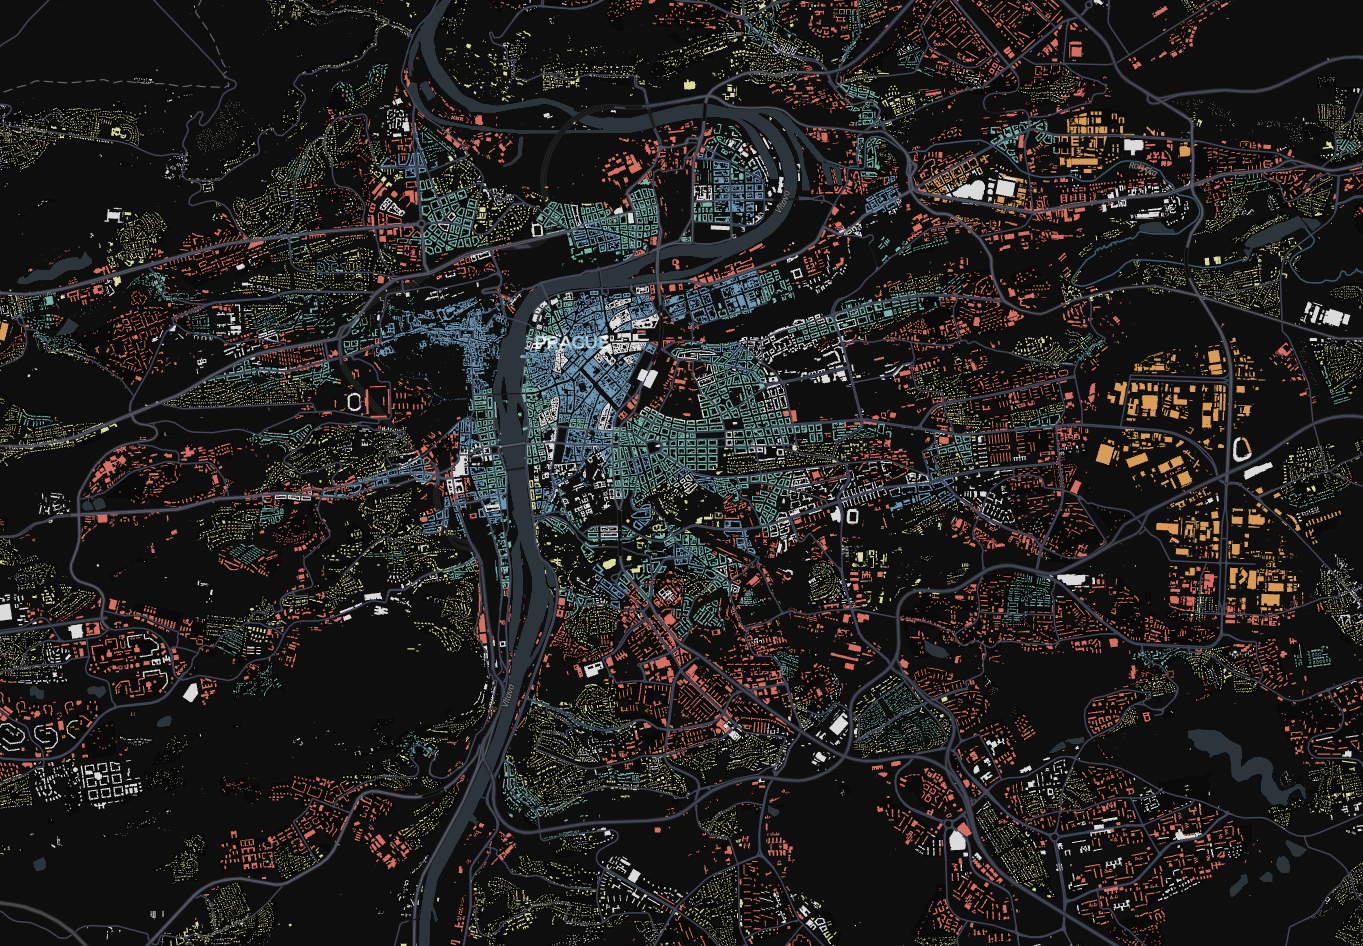
\includegraphics[width=\linewidth,height=4.16667in,keepaspectratio]{../figures/algo_design/prague_600.png}

}

\caption{High-level urban fabrics in Prague}

\end{figure}%

The second set breaks down each of the first sets into multiple subsets.
It goes into more detail and splits the houses into more classes, based
on features such as size and proximity to cities; it also splits the
historical areas based on origin - medieval, industrial-era and others;
the modern urban developments into subclasses such as different types of
modernist apartment blocks, commercial areas, offices and others; and
the several industrial area types. By analysing the model performance
across two different hierarchical levels, we will understand what is the
highest resolution detail the model can predict, given the shortcomings
of the data and which factors affect predictions.

\begin{figure}[H]

{\centering 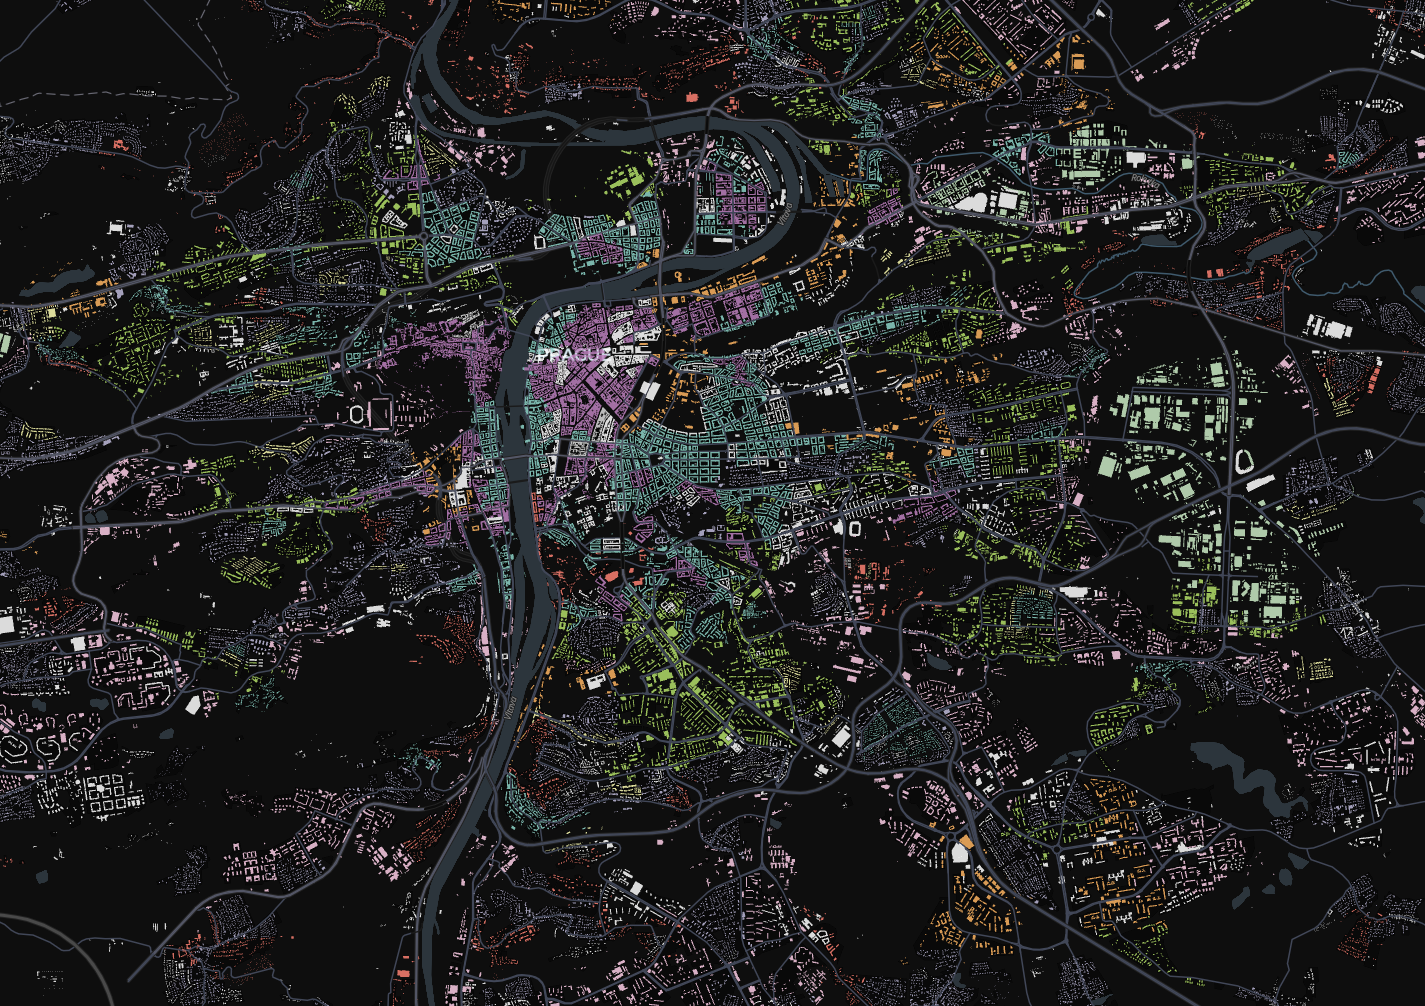
\includegraphics[width=\linewidth,height=4.16667in,keepaspectratio]{../figures/algo_design/prague_400.png}

}

\caption{More detailed urban fabrics in Prague}

\end{figure}%

\subsubsection{Prediction modelling and train/test
split}\label{prediction-modelling-and-traintest-split}

The main aim of the modelling task is to generate a classification of
morphological elements of similar quality to (Fleischmann and
Samardzhiev Forthcoming) given the data quality limitations, albeit
flat, not hierarchical. To achieve this we create an evaluation
framework for the selection of non-linear tree-based models like a
random forest classifier or an XGBoost model. We use the
satellite-derived buildings, their ETCs and their characteristics as
input data and the clusters from (Fleischmann and Samardzhiev
Forthcoming) as target labels for a classification task. The choice of
tree-based learning models is due to their readily available
implementations, high scalability and ability to quickly offer
interpretation insights. Furthermore, they handle well high dimensional
data, non-linear interactions and require minimal hyper-parameter
tuning. The flexibility of the models and the specific training/testing
framework setup will allow us to not just produce a predictive model but
also to identify potential areas for improvement in the original data
preprocessing.

Since we want the final production model to be general and applicable to
large areas i.e.~whole continents, it needs to be able to handle
previously unseen urban fabric types. For example, an urban morphology
type that is present in the test data, or in another study area, might
not be present in the training data and in that case the model should
flag its predicted label as uncertain. This is another area where tree
models have an advantage, since they are ensemble methods and this can
help reduces their tendency to overfit. They also readily provide a
confidence score for each prediction which can be used to flag unseen
data. Furthermore, we take extra care to evaluate the final production
models performance in realistic scenarios and the relationship between
its accuracy on test data and whole countries that are not part of the
model training or test data.

To achieve this we split the study area into five subsets and train five
independent iterations of each model. This is done so that that every
country and every combination of countries is used as final hold-out
test data and training/validation pipeline respectively. For example,
one iteration will use Germany, Poland, Czechia and Austria as part of
its training/validation pipeline, whereas Slovakia will be used as the
hold-out data.

\begin{figure}[H]

{\centering 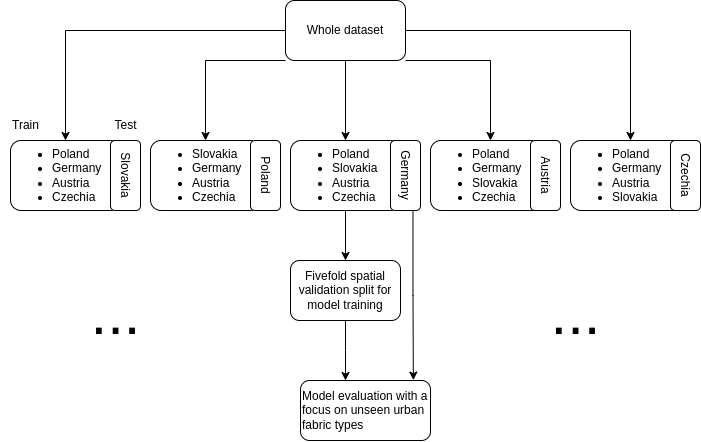
\includegraphics[width=\linewidth,height=4.16667in,keepaspectratio]{../figures/algo_design/eval_split.png}

}

\caption{Model evaluation and training setup}

\end{figure}%

This strategy acts as an extra check against overfitting and ultimately
enable us to see how the final production model will perform in
realistic scenarios - applying it to whole countries which are not used
for the training or testing at all. This comes with at least two
advantages over simply reporting a test score on a random sample. First,
it is a test of model performance on a dataset that does not have any
spatial leakage with the training or testing data. Second, it ensures
that we evaluate model performance on unseen urban fabric types from
other countries. We can afford to do this in part due to the large size
of the data we are working with. In every permutation there will be a
rich variety of urban fabrics and tens of millions of ETCs used in the
model training.

\subsubsection{Training and evaluation}\label{training-and-evaluation}

Lastly, after splitting the study area into five subsets, we create a
schema that will dictate how to split the training data of each subset
for the classification task. We use five-fold cross validation for hyper
parameter tuning, based on spatial contiguity. Random subsetting does
not work for this study, since we need to account for spatial dependency
and the related data leakage between train and evaluation data. The
spatial leakage comes from both the nature of the data - spatial
contiguity is one of the core aspects of morphological elements - but
also from the way characters are calculated based on various nearest
topological neighbours.

To account for this, we aggregate nearby ETCs into higher granularity
spatial units - level 7 H3 cells - and randomly split these units into
five groups, to carry out the cross-validation training. This ensures
that the majority of the ETCs and their neighbours in one set are not
present in the other sets, and therefore spatial leakage is minimised.
We use level 7 H3 cells, which represent a delineation of the globe into
hexagons with an area of approximately 5 sq. km. , rather than
enclosures or ETC contiguity, to ensure that contiguous subsets of test
data cover areas of heterogenous elements and present the model with a
realistic validation scenario.

\begin{figure}[H]

{\centering 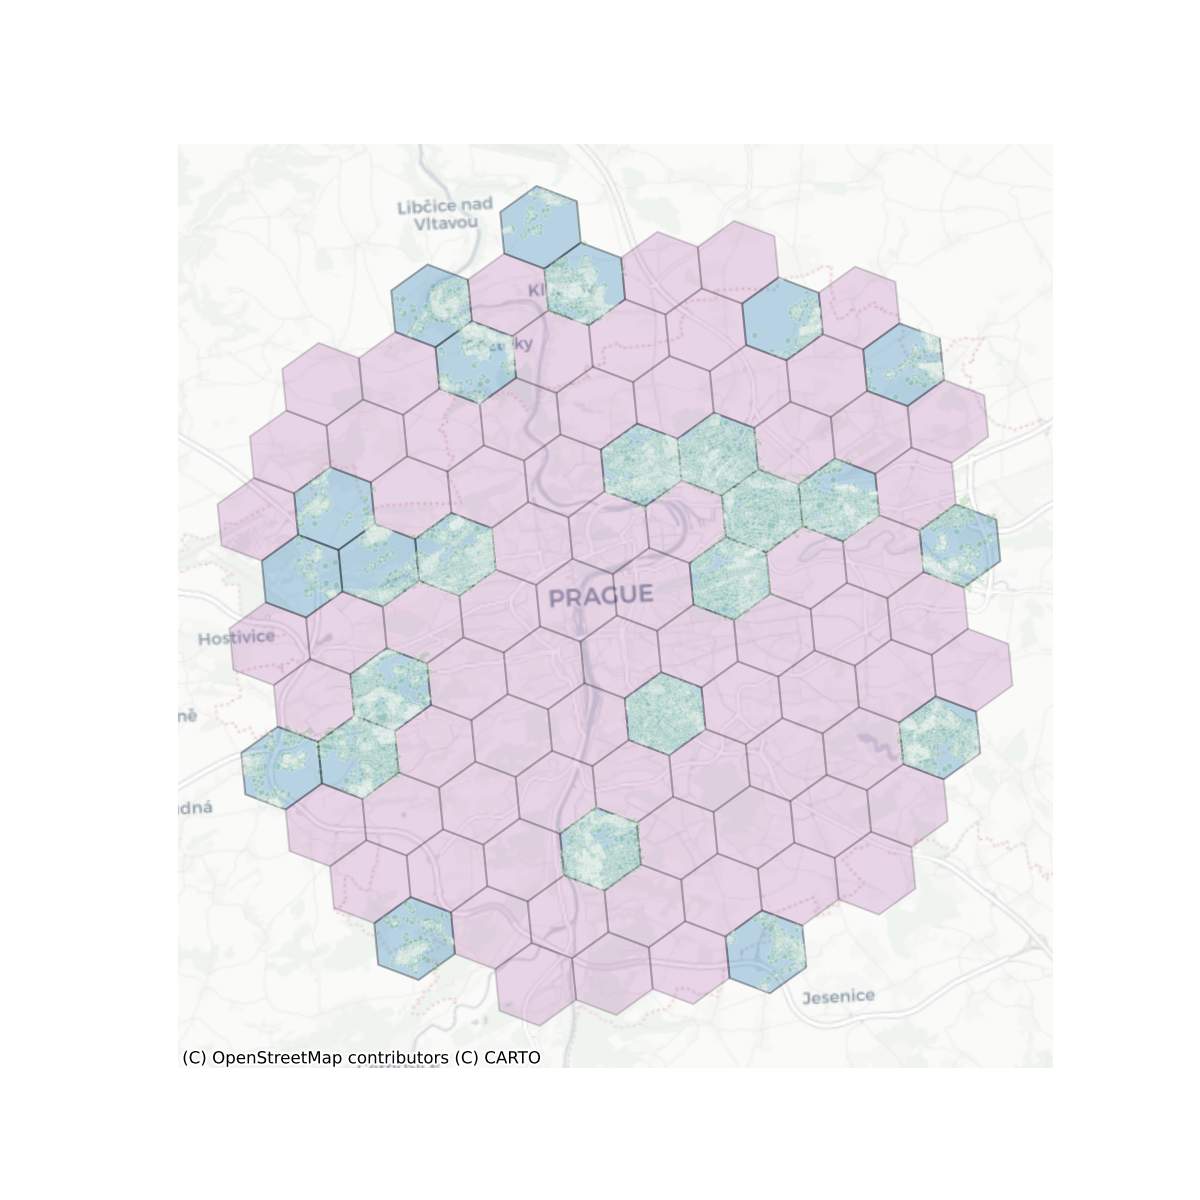
\includegraphics[width=\linewidth,height=4.16667in,keepaspectratio]{../figures/algo_design/train_test_prague.png}

}

\caption{Example iteration in a five-fold cross validation split. Only
one group is highligted in blue, with its ETCs plotted in green, which
will be used as a hold-out data for accuracy evaluation and hyper
parameter tuning.}

\end{figure}%%
\begin{figure}[H]

{\centering 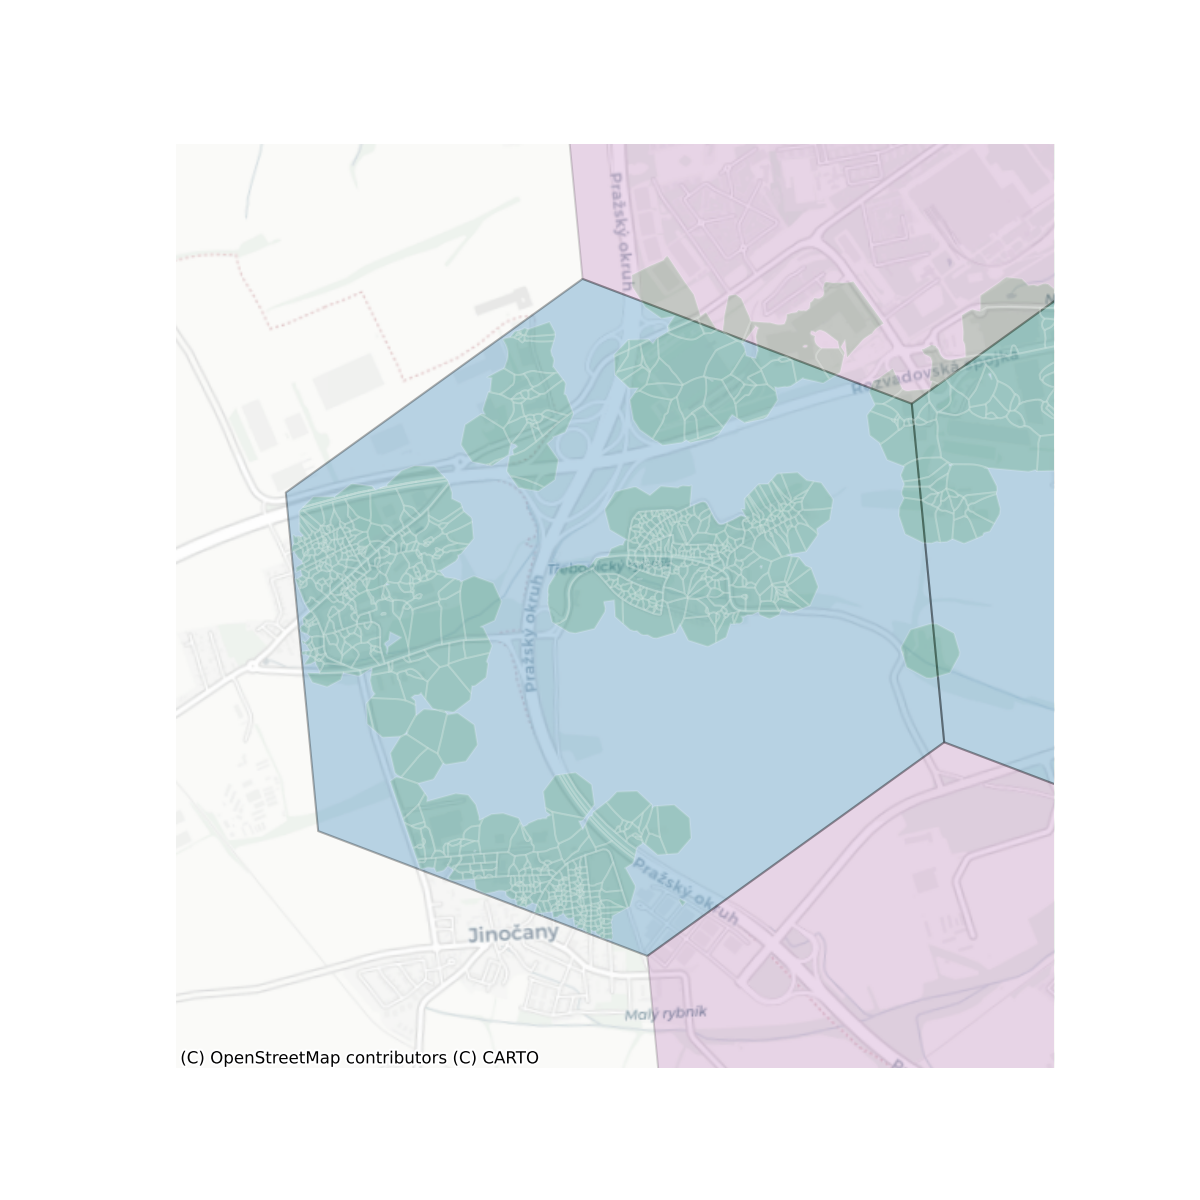
\includegraphics[width=\linewidth,height=4.16667in,keepaspectratio]{../figures/algo_design/train_test_prague_zoom2.png}

}

\caption{Example hexagon in the validation split}

\end{figure}%

The model training and evaluation will follow standard best practices -
model coefficients and hyper parameter tuning, such as the decision
threshold will be optimised based on the training subset, and all of the
data in the hold-out country will be used to give a final model accuracy
score. Specifically, the models will use balanced accuracy as the
optimisation metric in order to account for imbalances in the
distribution of urban fabric classes. The extra validation steps we
carry out with the hold-out countries will be used to used in three
ways. First, to contextualise the final models' accuracy on the test
data; second, to indicate how the model will perform on other countries;
and third to see how it handles urban fabric types not seen in the
training in a realistic scenario.

The final production model is trained on the whole dataset, using the
same hyper parameter grid search configuration and training/test spatial
split.

\subsubsection{Preliminary results}\label{preliminary-results}

We have implemented a preliminary pipeline that carries out full data
preprocessing - generating morphological elements and characters,
assigning target labels and some exploratory modelling. The core
functionality for all of this was made available within open-source
packages - \texttt{momepy}, \texttt{libpysal}, \texttt{sgeop} (the name
of which may eventually change).

Based on the preliminary results, there are 56,845,150 Microsoft
building footprints for our study area, which are split into 474
subregions. This is significantly less than the available cadastre data,
which has around 88 million buildings and are separated into 828
regions. The number of downloaded, unprocessed streets is similar to
those in (Fleischmann and Samardzhiev Forthcoming) - 23,332,865 - since
they cover the same study area and come from the same source - Overture
Maps, which is a processed subset of OpenStreepMap. However, the number
of tessellation cells is the same as the buildings and therefore less
than the cadastre data-based classification. Furthermore, the street
simplification algorithm is affected by the available buildings, and
therefore in turn also affects the tessellation cell boundaries.

These results highlight the effect of the satellite derived building
footprints that have been discussed in the Technical Note D3 . There are
significantly less subregions in the study area primarily due to the
effect of the threshold of 10k buildings required for a region. As the
adjacent buildings tend to be merged, the algorithm needs to cover
larger area before reaching the threshold, resulting in the lower number
of regions. However, as the region split is purely procedural step
allowing efficient processing of data, this is not an issue of any sort.

As a first modelling step we tried a random forest (RF) classifier on a
subset of the data covering the region surrounding Prague. The goal was
to evaluate the project workflow and the feasibility of the proposed
model architecture, rather than the specific model's performance. We
trained and tested the same simple RF model on the data within the same
region, split in different ways - one was based on stratified spatial
k-fold train/test splits (our proposed setup) and another based on
random train/test splits. The latter model with random sampling had an
accuracy of 0.95 versus an accuracy of 0.68 for the former model with
spatial stratification. The difference in accuracy highlights the extent
of spatial leakage of information and the need for the proposed
spatially explicit train/test/validation split of the data. Otherwise,
the performance of the production model would be significantly lower
than what the training data suggest. In any case, the relatively high
accuracy score of the models hint towards the viability of predicting
urban fabric types.

In total, the results point towards two things. First, they further show
need for a non-linear classification model, cable of accounting for the
discrepancies between satellite-derived building footprint and cadastral
data. Second, the utility of our designed framework to account for
spatial leakage and evaluate model performance in more realistic
scenarios.

\subsection{AI Modelling using Satellite
Imagery}\label{ai-modelling-using-satellite-imagery-1}

In satellite image analysis, classification and segmentation address
spatial labelling at different levels of granularity, with
classification assigning a single label to an image tile or cell, while
segmentation provides pixel-level detail. In our study, the label
dataset does not always correspond directly to identifiable features in
the imagery, making classification a potentially more suitable approach
as it generalises each tile's dominant land cover type without requiring
exact pixel alignment. However, we explore both approaches:
classification for a tile-based analysis and segmentation for finer,
boundary-specific mapping. This dual approach enables us to evaluate how
each method performs given the scale and nature of the dataset.

\subsubsection{Data preprocessing}\label{data-preprocessing-1}

For our analysis, we employ two distinct datasets of image tiles at
varying scales. These datasets enable us to evaluate both segmentation
and classification tasks for urban fabric prediction. We choose a larger
tile size for the segmentation task since most segmentation models work
better with conventional image sizes (such as 224 x 224 pixels) and they
are also a lot more efficient since the dataset is not as large. For
classification, the tile size represents the scale of the analysis and
for that reason we chose a smaller tile size of 56x56 pixels.

\begin{itemize}
\tightlist
\item
  \textbf{Segmentation Dataset}: Comprising 26,753 tiles, each 224 x 224
  pixels (covering 2240 x 2240 meters). Of these, 21,402 tiles are
  allocated for training, and 5,351 for testing.
\item
  \textbf{Classification Dataset}: Comprising 403,722 tiles, each 56 x
  56 pixels (covering 560 x 560 meters). The training set consists of
  342,648 tiles, with the remaining 61,074 reserved for testing.
\end{itemize}

To ensure consistency across both tasks, we exclusively use tiles that
fully overlap with the spatial signature labels. This alignment
facilitates robust pixel-level comparisons of classification and
segmentation outcomes while maintaining compatibility with our urban
fabric typology as shown below.

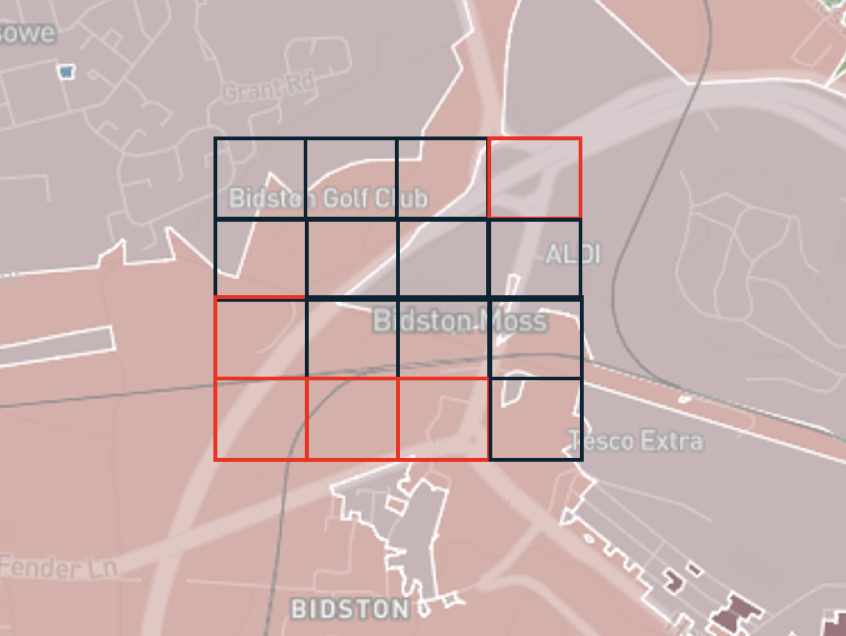
\includegraphics[width=\linewidth,height=4.16667in,keepaspectratio]{../figures/algo_design/sampling.png}\hfill

\paragraph{Unbalanced dataset}\label{unbalanced-dataset}

A significant challenge in our dataset is class imbalance, where certain
urban fabric types are much more prevalent than others. This imbalance
required careful consideration in model design and loss function
selection, prompting us to explore approaches that could better handle
uneven class distributions.

The figure below visualizes the class distribution of spatial
signatures, highlighting the imbalance across different urban fabric
types. Notably, the countryside agriculture and wild countryside classes
are more dominant compared to the more urban-centric classes.

\begin{center}
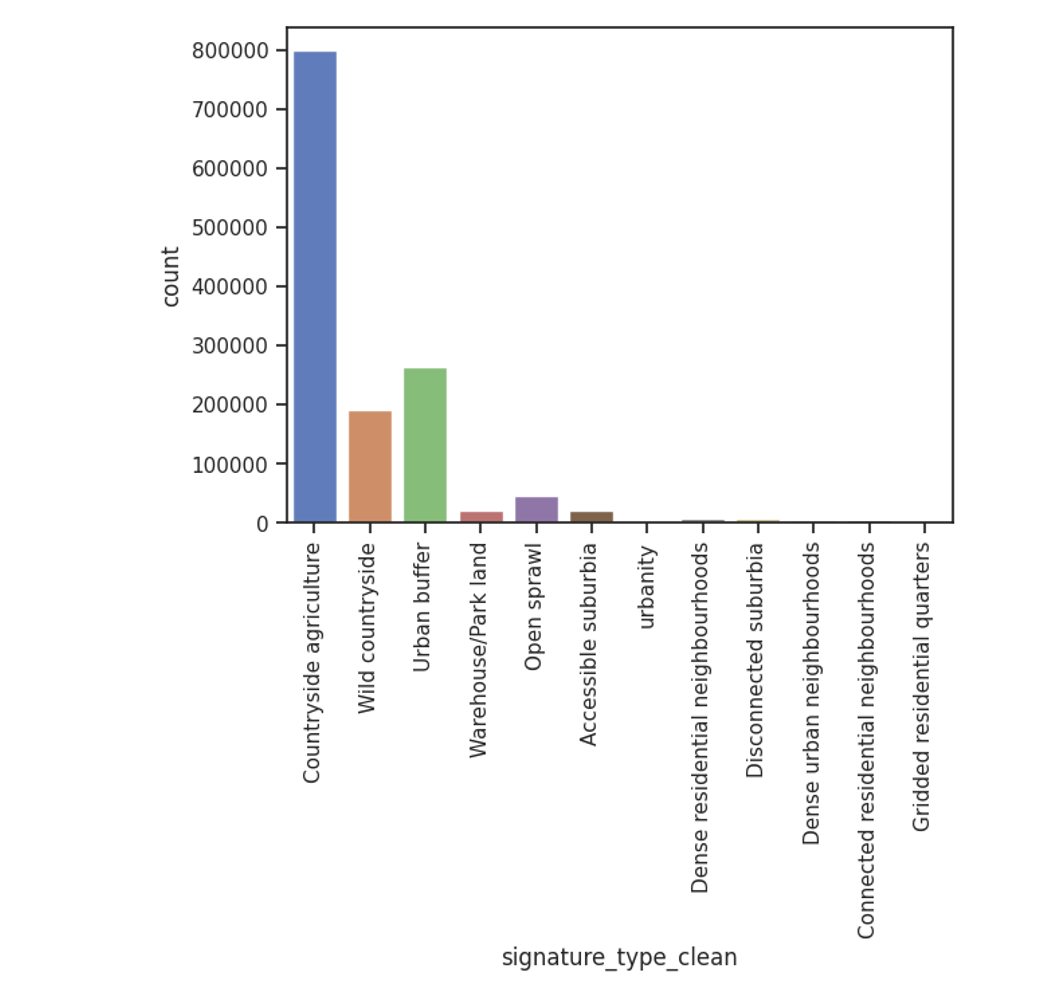
\includegraphics[width=\linewidth,height=4.375in,keepaspectratio]{../figures/algo_design/unbalanced.png}
\end{center}

\paragraph{Train/test split}\label{traintest-split}

The dataset is divided into 80\% for training and 20\% for testing
across both tasks. The segmentation and classification datasets share
the same test samples, which helps make the results more comparable and
allows us to evaluate performance across both tasks at the same time.

The figures below show how the training and testing datasets sampled
across the whole study area:

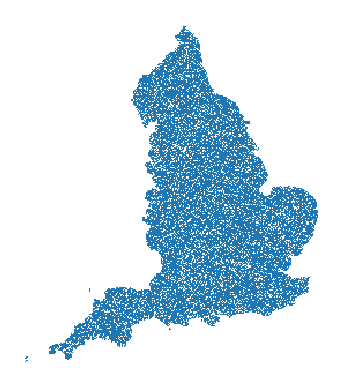
\includegraphics[width=\linewidth,height=4.16667in,keepaspectratio]{../figures/algo_design/train_df.png}\hfill
\hfill
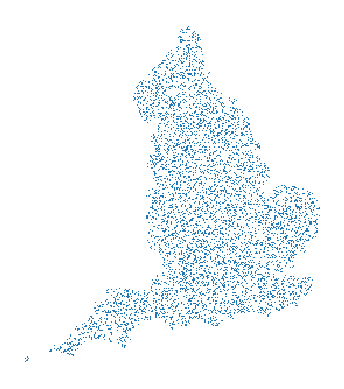
\includegraphics[width=\linewidth,height=4.16667in,keepaspectratio]{../figures/algo_design/test_df.png}

We used standard, pre-configured neural network setups without tuning
the hyperparameters, due to the constraints of the project. As a result,
we did not include a validation split in these experiments.

\subsubsection{Model architectures}\label{model-architectures}

To assess the performance of different AI models for urban fabric
classification and segmentation, we designed three distinct experimental
approaches. Each approach leverages different combinations of
pre-trained models and fine-tuning strategies to evaluate their ability
to accurately classify and segment urban fabric types. The following
experiments were carried out to explore the effectiveness of both image
embeddings and geospatial foundation models in addressing the challenges
posed by urban fabric analysis:

We conducted three main experiments as part of the AI model design to
analyze urban fabric classification and segmentation.

\begin{itemize}
\item
  Approach A (\emph{Embedding approach}): We start with a baseline
  experiment, where we generate image embeddings using the
  SatlasPretrain model. These embeddings are then fed into an XGBoost
  classifier to predict urban fabric classes.
\item
  Approach B (\emph{Segmentation approach}): Next, we fine-tune three
  different geospatial foundation models---SatlasPretrain, Clay, and
  IBM/NASA's Prithvi model---specifically for segmentation tasks.
\item
  Approach C (\emph{Classification approach}): Finally, we take the
  best-performing geospatial foundation model from the segmentation
  experiments (Clay) and fine-tune it for the classification task.
\end{itemize}

To evaluate and compare the results of these approaches, we report
weighted pixel-level accuracy, F1 score, and Intersection over Union
(IoU) metrics.

\paragraph{Baseline embedding approach (Approach
A)}\label{baseline-embedding-approach-approach-a}

In the first experiment, we implement a baseline approach using image
embeddings created by a geospatial foundation model, followed by
classification with an XGBoost model. This approach is computationally
efficient and easy to implement, making it a good starting point for
comparison. Once the embeddings are generated, they can be directly
input into a machine learning (ML) model for classification.

The tiles are processed by the SatlasPretrain model (Bastani et al.
2023), a geospatial foundation model pretrained on more than 302 million
labels from remote sensing and computer vision tasks. We chose this
model because it was specifically trained on Sentinel-2 images, making
it a good fit for our dataset.

The model works in two steps:

\begin{itemize}
\tightlist
\item
  Foundation Model: We use a Vision Transformer (ViT) with a Feature
  Pyramid Network (FPN) and a pooling layer to generate image
  embeddings. These embeddings are lower-dimensional representations of
  the images.
\item
  Machine Learning Classifier: The generated embeddings are then passed
  into an XGBoost classifier, which predicts the urban fabric classes
  across England.
\end{itemize}

The diagram below illustrates this baseline approach: \begin{center}
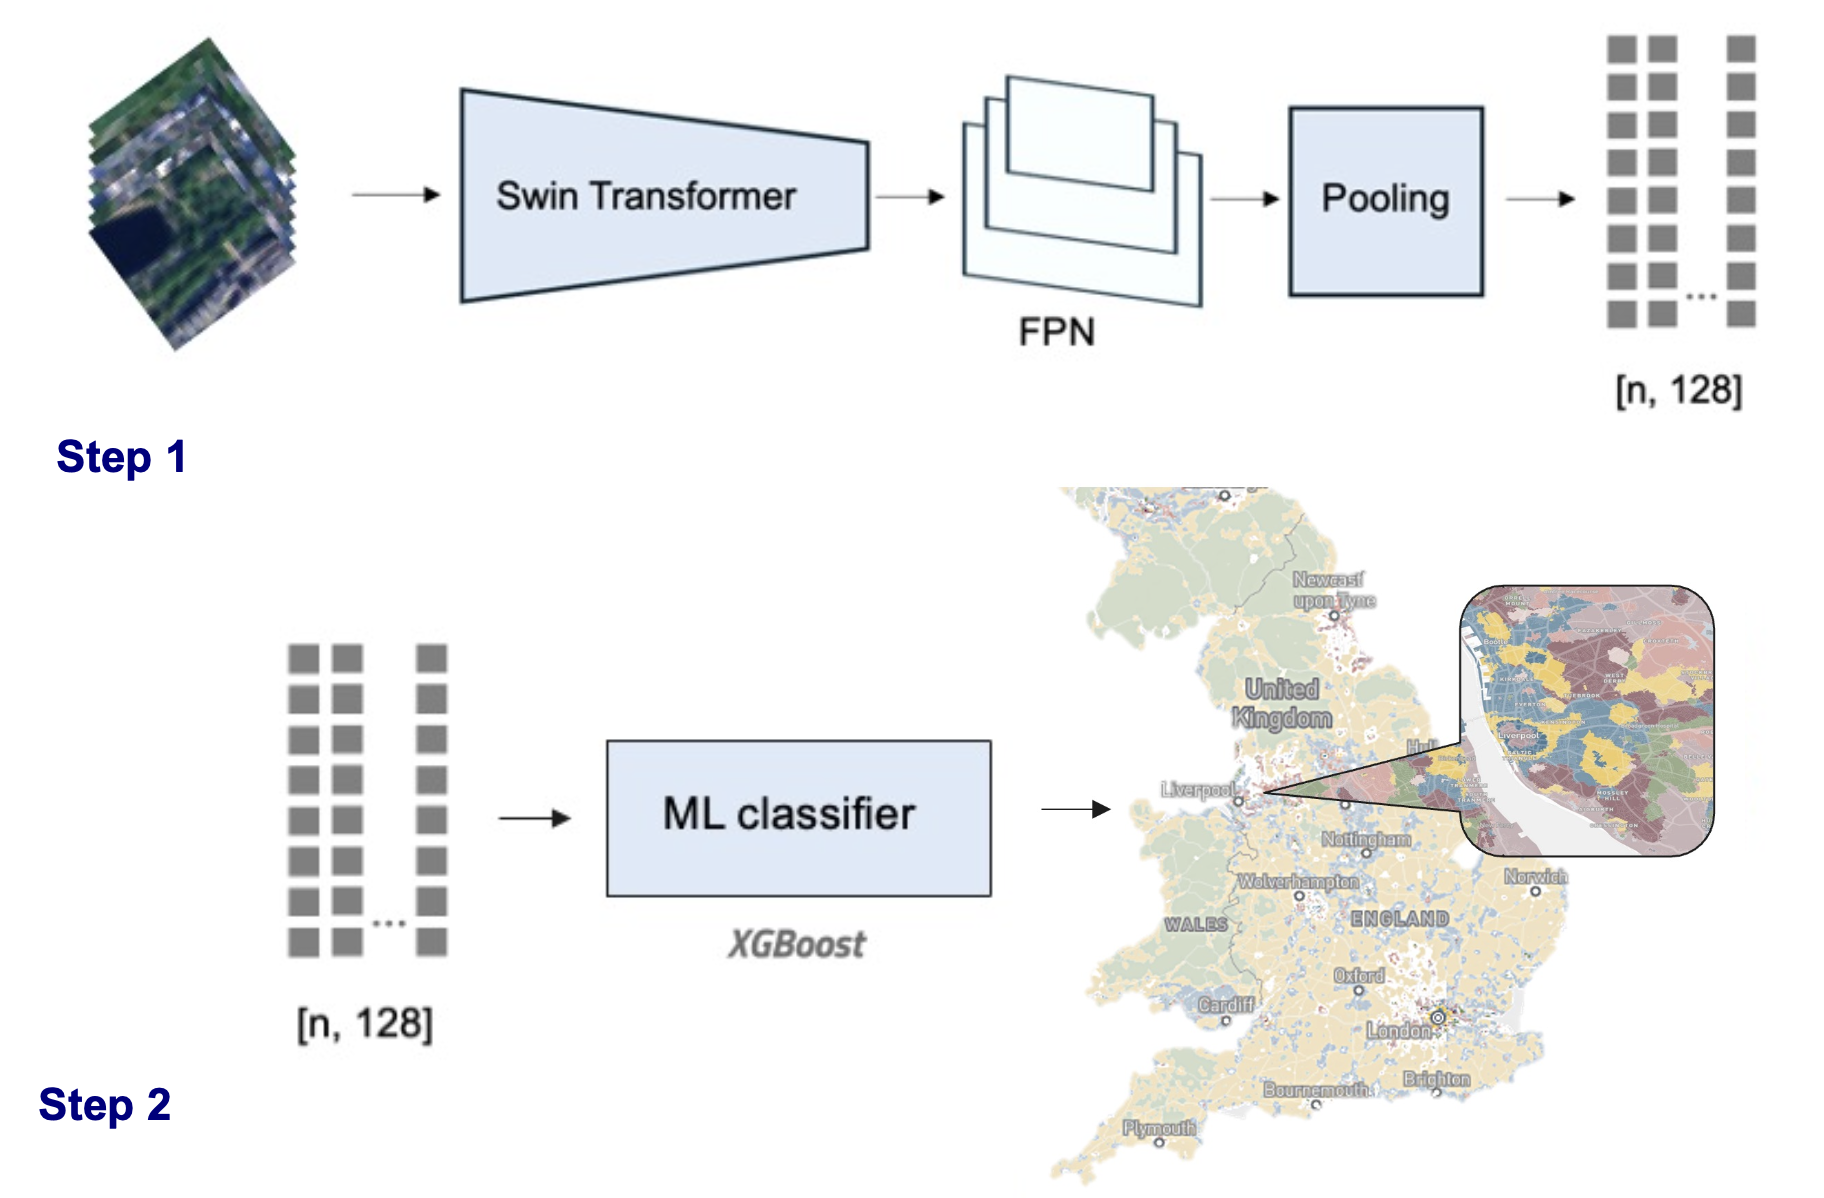
\includegraphics[width=\linewidth,height=4.16667in,keepaspectratio]{../figures/algo_design/baseline.png}
\end{center}

\emph{Baseline approach (ordinal)}

In addition to the basic classification task, we also explored an
ordinal regression approach. Since the urban fabric classes represent a
continuum rather than strictly categorical data, this approach accounts
for the ordering between the classes. The following ordinal mapping was
applied to model the spatial signatures:

\texttt{ordinal\_mapping\ =\ \{\ \ \ \ \ \textquotesingle{}Wild\ countryside\textquotesingle{}:\ 0,\ \ \ \ \ \textquotesingle{}Countryside\ agriculture\textquotesingle{}:\ 1,\ \ \ \ \ \textquotesingle{}Urban\ buffer\textquotesingle{}:\ 2,\ \ \ \ \ \textquotesingle{}Open\ sprawl\textquotesingle{}:\ 3,\ \ \ \ \ \textquotesingle{}Disconnected\ suburbia\textquotesingle{}:\ 4,\ \ \ \ \ \textquotesingle{}Accessible\ suburbia\textquotesingle{}:\ 5,\ \ \ \ \ \textquotesingle{}Warehouse/Park\ land\textquotesingle{}:\ 6,\ \ \ \ \ \textquotesingle{}Gridded\ residential\ quarters\textquotesingle{}:\ 7,\ \ \ \ \ \textquotesingle{}Connected\ residential\ neighbourhoods\textquotesingle{}:\ 8,\ \ \ \ \ \textquotesingle{}Dense\ residential\ neighbourhoods\textquotesingle{}:\ 9,\ \ \ \ \ \textquotesingle{}Dense\ urban\ neighbourhoods\textquotesingle{}:\ 10,\ \ \ \ \ \textquotesingle{}Urbanity\textquotesingle{}:\ 11,\ \}}

Using this ordinal mapping, the model achieved a Mean Absolute Error
(MAE) and Mean Squared Error (MSE) of 0.28, with an R² score of 0.62.
The Sankey diagram below shows the main misclassifications, which
typically occur between similar urban fabric types.

\begin{center}
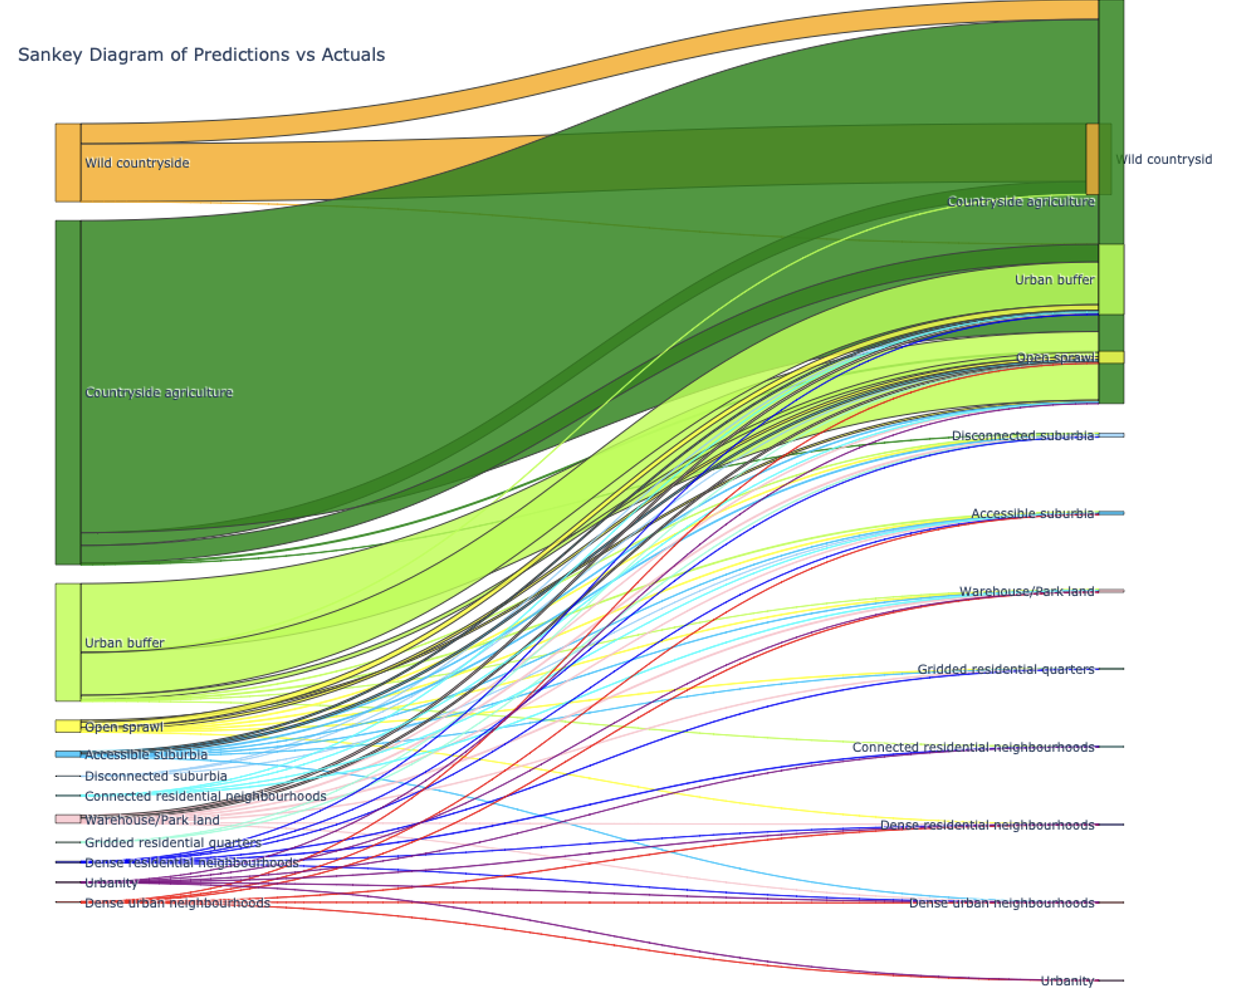
\includegraphics[width=\linewidth,height=4.375in,keepaspectratio]{../figures/algo_design/sankey.png}
\end{center}

For pixel-level comparison, we round the predicted values to the closest
class and report them in the overview in the Preliminary results
section.

\emph{Baseline approach + spatial context}

To further improve model performance, we added spatial context by
including regional geographical information to the predictive model. We
thus added the regional H3 resolution 5 code as categorical variable to
the machine learning models. The visualisation below shows the hexagons
plotted on top of England.

\begin{center}
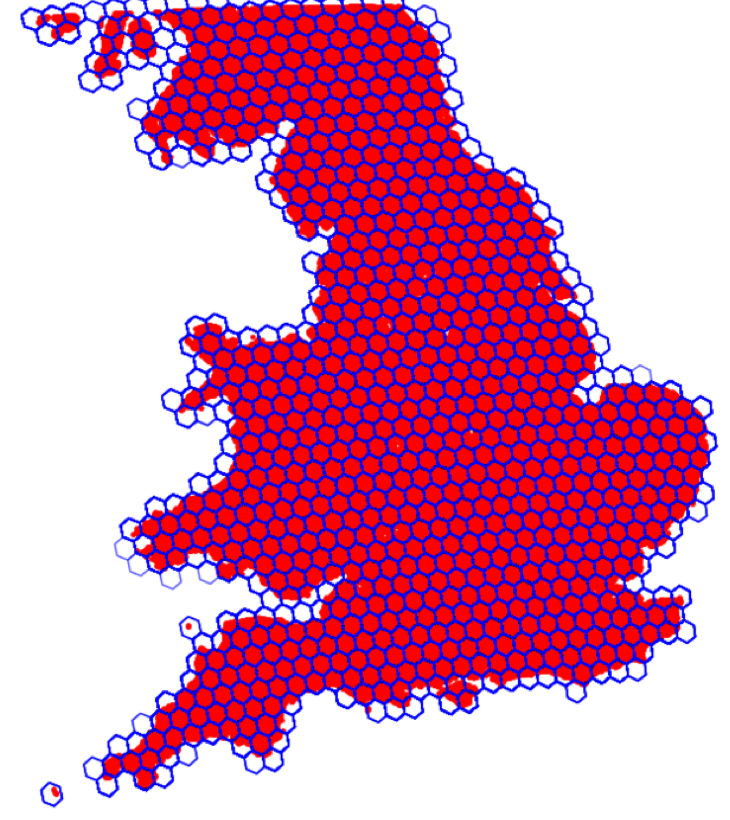
\includegraphics[width=\linewidth,height=4.375in,keepaspectratio]{../figures/algo_design/hex_level5.png}
\end{center}

\paragraph{Segmentation (Approach B)}\label{segmentation-approach-b}

In this section, we explore segmentation using a fine-tuned geospatial
foundation model. We trained three state-of-the-art models on 224x224x3
image tiles to classify urban fabric types at a pixel level. Each model
was fine-tuned for 10 epochs, and we evaluated their performance using
key metrics. The models we tested vary in architecture and dataset size,
as summarized below:

\begin{longtable}[]{@{}llll@{}}
\toprule\noalign{}
Model & Architecture & Dataset Size & Image Sources \\
\midrule\noalign{}
\endhead
\bottomrule\noalign{}
\endlastfoot
Satlas \footnote{https://huggingface.co/allenai/satlas-pretrain} & SwinT
& 302M labels & Sentinel-2 \\
Clay \footnote{https://huggingface.co/made-with-clay/Clay} & MAE/ViT &
70M labels & Multiple+ \\
Prithvi \footnote{https://huggingface.co/ibm-nasa-geospatial/Prithvi-100M}
& MAE/ViT & 250 PB & Sentinel-2/Landsat \\
\end{longtable}

+Multiple sources include Sentinel-2, Landsat, NAIP, and LINZ

These models differ mainly in their backbone architecture and the
datasets they were pretrained on, which impacts their ability to capture
different spatial and spectral features from the input images.

The following visualisations show the varying model configurations for
the three different approaches tested for the segmentation task. The
main difference is the varying backbone.

\paragraph{Model 1: Satlas}\label{model-1-satlas}

\begin{center}
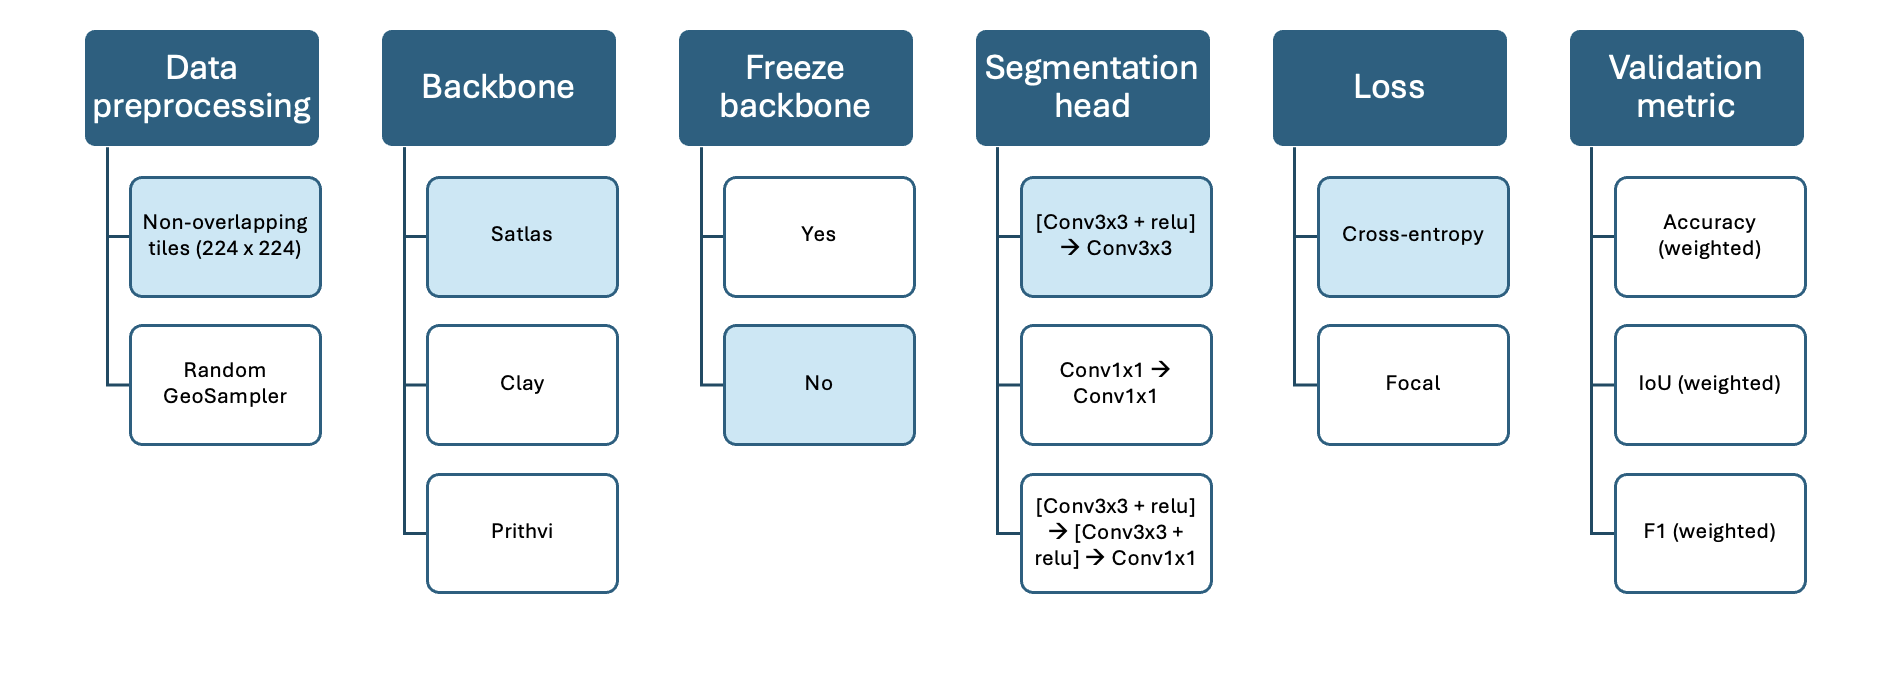
\includegraphics[width=6.25in,height=\textheight,keepaspectratio]{../figures/algo_design/satlas_model.png}
\end{center}

\paragraph{Model 2: Clay}\label{model-2-clay}

\begin{center}
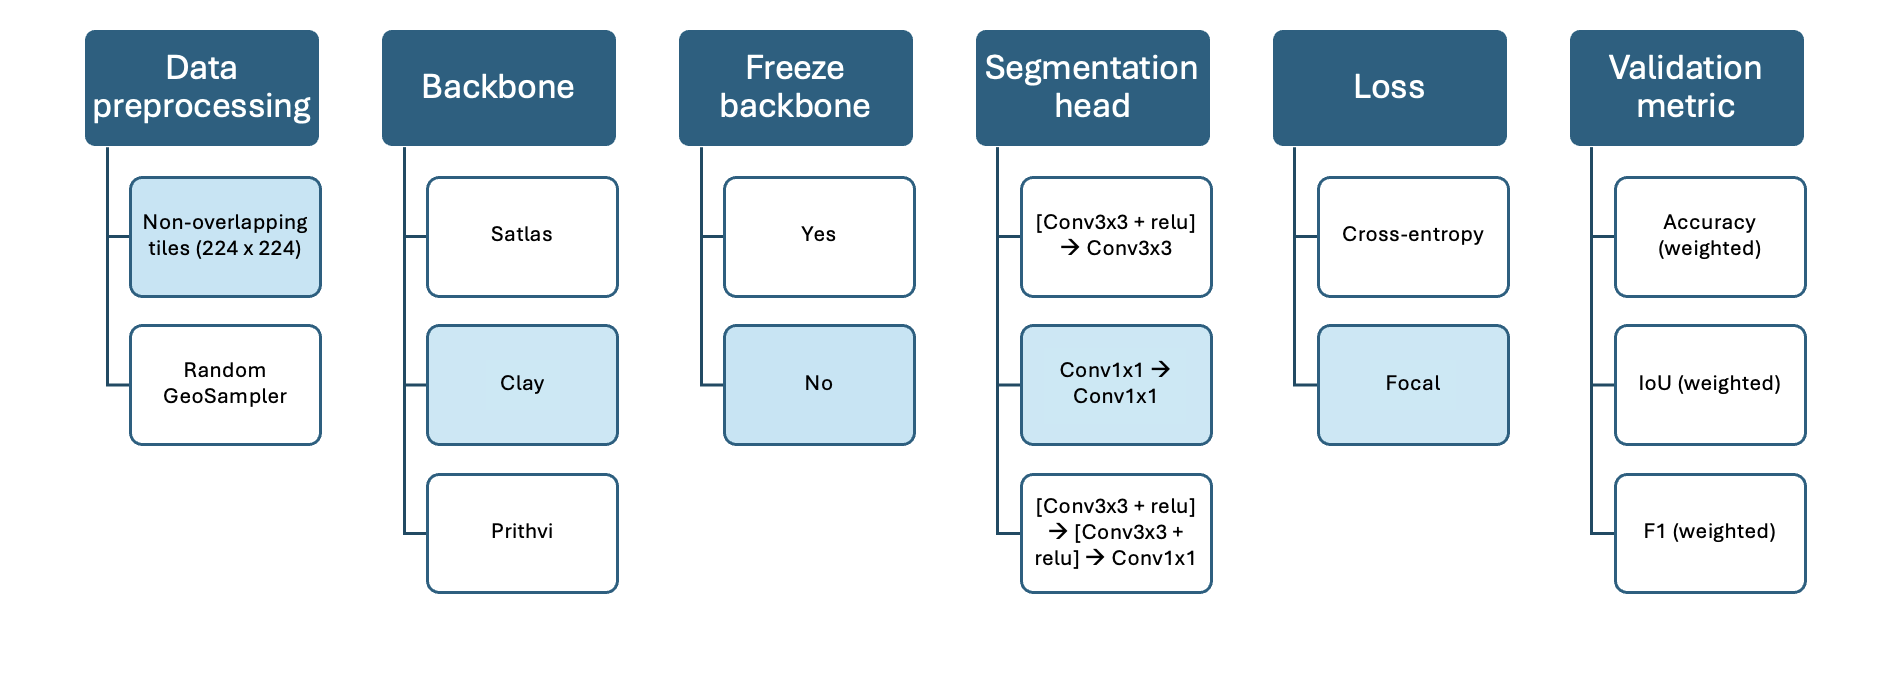
\includegraphics[width=6.25in,height=\textheight,keepaspectratio]{../figures/algo_design/clay_model.png}
\end{center}

\paragraph{Model 3: Prithvi}\label{model-3-prithvi}

\begin{center}
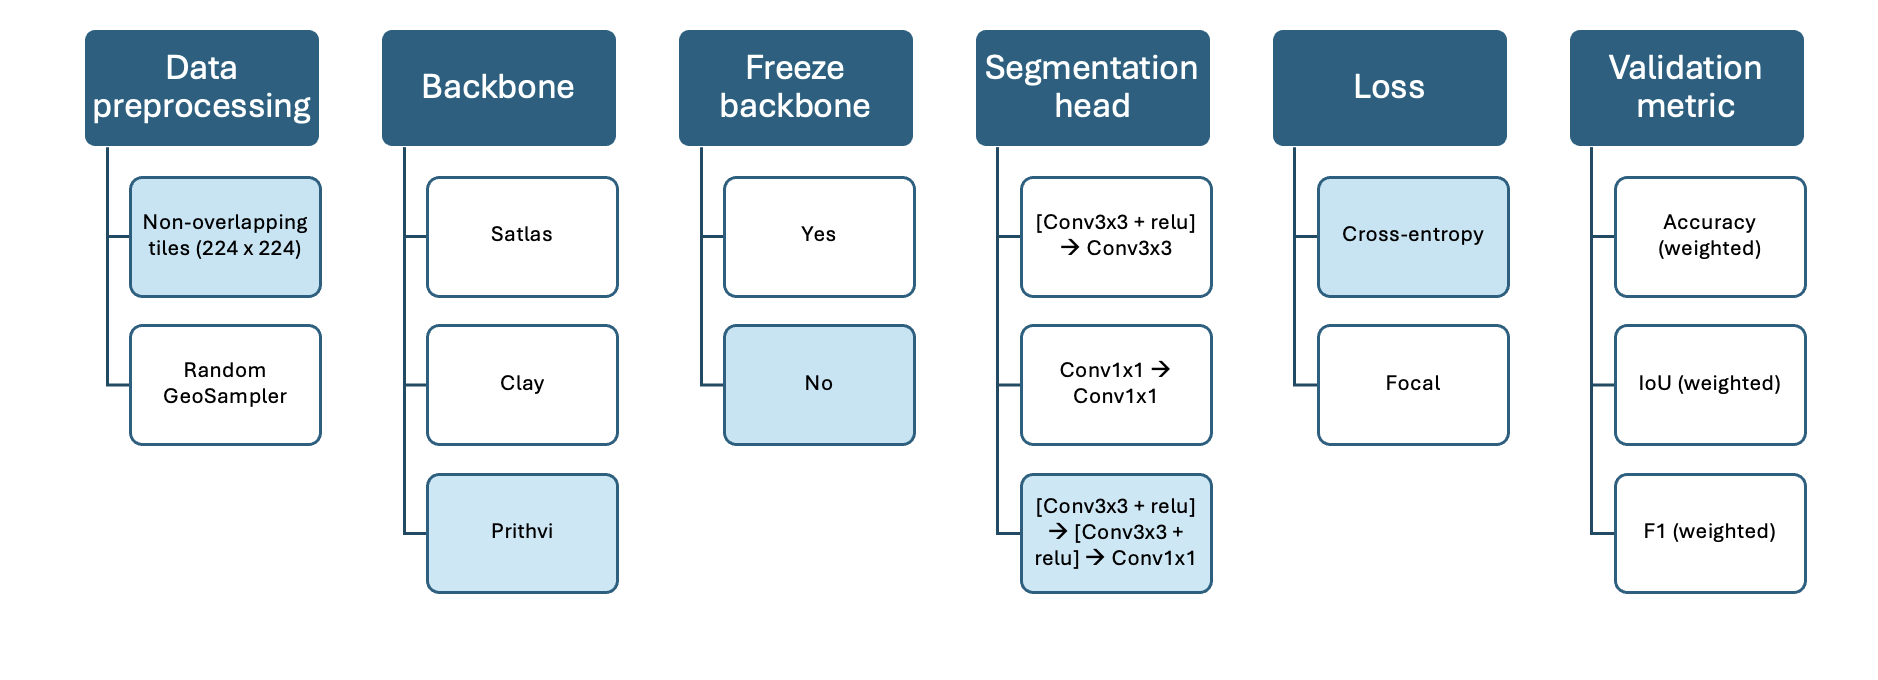
\includegraphics[width=6.25in,height=\textheight,keepaspectratio]{../figures/algo_design/prithvi_model.png}
\end{center}

After fine-tuning each model for 10 epochs, we compared their
performance based on weighted accuracy, Intersection over Union (IoU),
and F1 score, among other metrics. The table below summarizes the
results of the segementation model comparison:

\begin{longtable}[]{@{}llll@{}}
\toprule\noalign{}
Metric & Satlas & Clay & Prithvi \\
\midrule\noalign{}
\endhead
\bottomrule\noalign{}
\endlastfoot
Weighted Accuracy & 0.57 & \textbf{0.72} & 0.62 \\
Weighted IoU & 0.33 & \textbf{0.58} & 0.41 \\
Weighted F1 & 0.41 & \textbf{0.69} & 0.58 \\
Training Time/Epoch & 9 mins & 8 mins & 20 mins \\
Parameters & 90M & 86M & 120M \\
Implementation Score & 5/10 & 6/10 & 7/10 \\
\end{longtable}

The Clay model outperformed the others across all metrics, demonstrating
the best performance in terms of weighted accuracy, IoU, and F1 score,
while maintaining reasonable training times and computational
efficiency.

The choice of loss function played a crucial role in the performance of
the models. We found that focal loss was particularly effective in
handling class imbalance, a common challenge in geospatial datasets.
When applied with the Clay model, this loss function led to significant
improvements in segmentation accuracy, especially for underrepresented
urban fabric classes.

\paragraph{Classification (Approach C)}\label{classification-approach-c}

In Approach C, we focused on fine-tuning a geospatial foundation model
for a classification task. For this, we used the smaller 56x56x3 image
tiles as input. Based on the promising results from the segmentation
experiments (Approach B), we chose to use the Clay model as the backbone
for this classification task, as it consistently outperformed the other
models across key metrics.

The figure below compares the predicted urban fabric classes from the
fine-tuned geospatial foundation model in both the segmentation
(Approach B) and classification (Approach C) tasks. This visual
comparison highlights the differences in the model's performance and the
class predictions between these two approaches.

\begin{center}
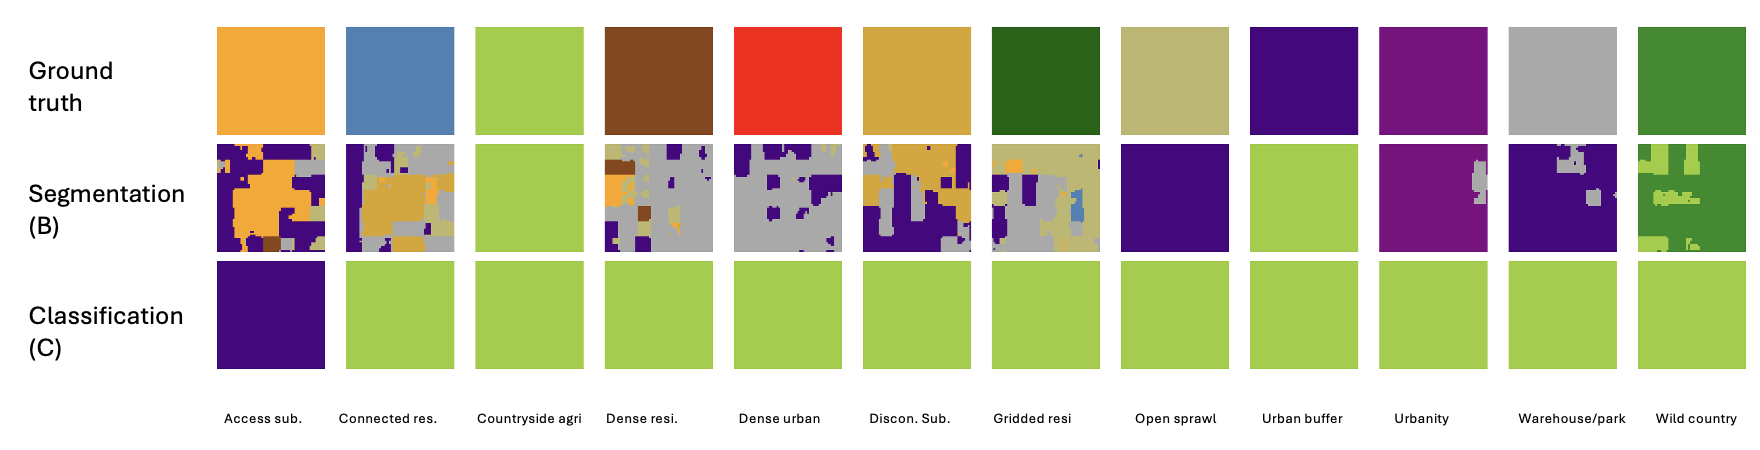
\includegraphics[width=6.25in,height=\textheight,keepaspectratio]{../figures/algo_design/comparison_B_C.png}
\end{center}

While the classification approach (Approach C) tends to overpredict the
dominant class, the segmentation output from Approach B faces challenges
in representing useful shapes for classes with fewer examples. These
differences highlight the trade-offs in model performance across tasks
with varying data distributions. Additionally, this could suggest that
some spatial signatures lack clear boundaries on the ground, making it
difficult for the segmentation algorithm to accurately detect borders
between classes. This insight underscores the complexities of applying
segmentation techniques to spatial data with ambiguous or overlapping
class boundaries.

\subsubsection{Evaluation Metrics}\label{evaluation-metrics}

To comprehensively evaluate the performance of our models, we used
several key metrics that capture different aspects of model performance:

\begin{itemize}
\item
  Intersection over Union (IoU): This metric quantifies the overlap
  between predicted and ground truth segmentations. It ranges from 0 (no
  overlap) to 1 (perfect overlap). IoU is calculated by dividing the
  area of intersection by the area of the union between the predicted
  and actual segmentation masks.
\item
  Weighted F1 Score: The F1 score is the harmonic mean of precision and
  recall, offering a balanced measure of both. The weighted F1 score
  adjusts for class imbalances by giving more importance to classes with
  fewer examples. Precision measures how many of the predicted positives
  are correct, while recall indicates how many of the actual positives
  were correctly identified.
\item
  Weighted Accuracy: This metric measures the overall proportion of
  correct predictions, adjusted by class frequencies to address class
  imbalance. It provides a more representative performance measure by
  considering the prevalence of each class in the dataset.
\end{itemize}

\subsubsection{Preliminary results}\label{preliminary-results-1}

Comparing model results directly can be challenging due to differences
in image tile sizes and overlap (e.g., 56px vs.~224px). To ensure a fair
comparison, we calculate pixel-level accuracy scores for each approach.
Specifically, we predict the full map for the test set, compare
overlapping tiles (as described in the sampling method), and compute the
following metrics on a per-pixel basis.

\paragraph{Overall model performance comparison
(Pixel-level)}\label{overall-model-performance-comparison-pixel-level}

Our evaluation across the different approaches showed varying levels of
performance. Below is a summary of the performance metrics for each
approach:

\begin{longtable}[]{@{}
  >{\raggedright\arraybackslash}p{(\linewidth - 8\tabcolsep) * \real{0.1754}}
  >{\raggedright\arraybackslash}p{(\linewidth - 8\tabcolsep) * \real{0.2807}}
  >{\raggedright\arraybackslash}p{(\linewidth - 8\tabcolsep) * \real{0.2807}}
  >{\raggedright\arraybackslash}p{(\linewidth - 8\tabcolsep) * \real{0.1754}}
  >{\raggedright\arraybackslash}p{(\linewidth - 8\tabcolsep) * \real{0.0877}}@{}}
\toprule\noalign{}
\begin{minipage}[b]{\linewidth}\raggedright
Approach
\end{minipage} & \begin{minipage}[b]{\linewidth}\raggedright
Global Accuracy
\end{minipage} & \begin{minipage}[b]{\linewidth}\raggedright
Macro Accuracy
\end{minipage} & \begin{minipage}[b]{\linewidth}\raggedright
F1 Score
\end{minipage} & \begin{minipage}[b]{\linewidth}\raggedright
IoU
\end{minipage} \\
\midrule\noalign{}
\endhead
\bottomrule\noalign{}
\endlastfoot
A: Classification (embeddings) & 0.76 (0.66) & 0.22 (0.13) & 0.23 &
0.63 \\
A: Classification + H3 level 5 & \textbf{0.87} (0.82) & \textbf{0.42}
(0.35) & \textbf{0.45} & \textbf{0.79} \\
A: Classification + H3 ordinal & 0.80 (0.80) & 0.26 (0.26) & 0.26 &
0.69 \\
B: Segmentation (Clay) & 0.73 & 0.31 & 0.30 & 0.58 \\
C: Classification (Clay) & 0.59 (0.68) & 0.09 & 0.12 & 0.38 \\
\end{longtable}

The results in brackets represent the tile-level accuracy, which is
typically reported in classification tasks. However, to facilitate more
meaningful comparisons across approaches, we use pixel-level accuracy
for all experiments.

\textbf{Key observations}

\begin{itemize}
\item
  The baseline classification approaches showed varied results:

  \begin{itemize}
  \tightlist
  \item
    The basic embedding classification approach achieved a global
    accuracy of 76\% (22\% balanced), reflecting a strong initial
    performance.
  \item
    When incorporating regional trends, performance improved
    significantly, with a global accuracy of 87\% (42\% balanced),
    suggesting that regional context plays a critical role in improving
    classification accuracy.
  \item
    The H3 Level 5 ordinal classification approach also performed well,
    with an accuracy of 80\% (26\% balanced), but it lagged behind in
    balancing the performance across classes.
  \end{itemize}
\item
  The fine-tuned geospatial foundation model performed better than the
  fine-tuned classification models, achieving an accuracy of 0.73
  compared to 0.56 for the classification model (Clay model).
\item
  Overall, the classification approach with regional information (H3
  Level 5) yielded the best performance, achieving both high accuracy
  and a reasonable balance across classes. Additionally, this approach
  is computationally efficient: once the image embeddings are generated,
  the downstream classification process can be completed in just a few
  minutes.
\end{itemize}

\paragraph{Prediction example: London}\label{prediction-example-london}

To showcase the practical application of the model, we used it to make
predictions on a map of London. This example uses the model from
Approach A, which incorporates regional trends through H3 categories,
and generates predictions across the entire country. The figure below
presents a sample prediction for the London area, where each color
represents a different spatial signature, and the background color
corresponds to the ground truth.

\begin{center}
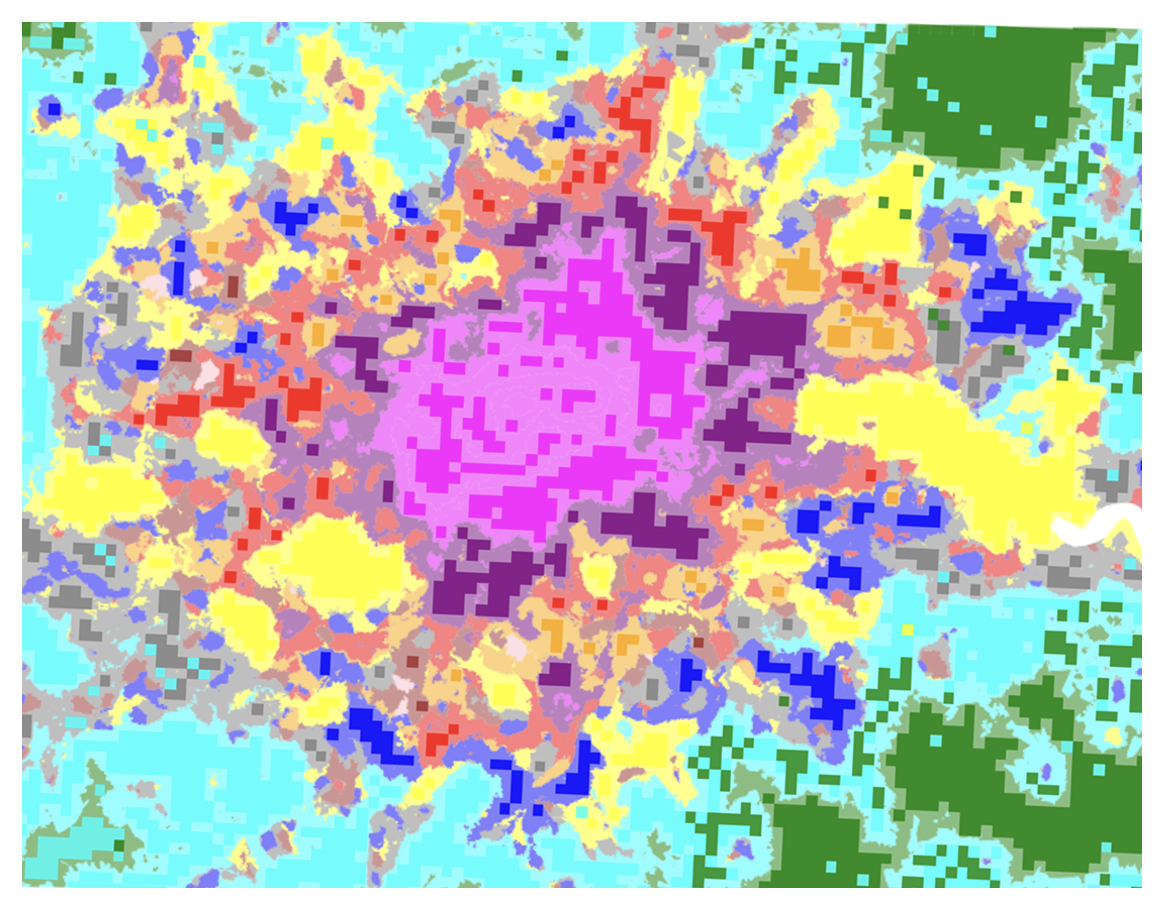
\includegraphics[width=\linewidth,height=4.375in,keepaspectratio]{../figures/algo_design/results_eurofab.png}
\end{center}

\subsubsection{25x25 grid classification
pipeline}\label{x25-grid-classification-pipeline}

Following the initial analysis, which demonstrated that the
embeddings-based approach yielded the most favorable results, we
extended the classification pipeline to include testing with a finer
grid resolution. Through team discussions, we determined that a grid
size of 25x25 pixels (corresponding to 250x250 meters on the ground) is
particularly well-suited for downstream planning applications. This
smaller grid size not only aligns better with practical use cases but
also led to improvements in key performance metrics such as the overall
weighted F1 score and macro accuracy. However, the overall accuracy is a
bit lower, which is for our application not as important.

\begin{longtable}[]{@{}
  >{\raggedright\arraybackslash}p{(\linewidth - 8\tabcolsep) * \real{0.1353}}
  >{\raggedright\arraybackslash}p{(\linewidth - 8\tabcolsep) * \real{0.3534}}
  >{\raggedright\arraybackslash}p{(\linewidth - 8\tabcolsep) * \real{0.1654}}
  >{\raggedright\arraybackslash}p{(\linewidth - 8\tabcolsep) * \real{0.1579}}
  >{\raggedright\arraybackslash}p{(\linewidth - 8\tabcolsep) * \real{0.1880}}@{}}
\toprule\noalign{}
\begin{minipage}[b]{\linewidth}\raggedright
\textbf{Tile size}
\end{minipage} & \begin{minipage}[b]{\linewidth}\raggedright
\textbf{Model}
\end{minipage} & \begin{minipage}[b]{\linewidth}\raggedright
\textbf{Global Accuracy}
\end{minipage} & \begin{minipage}[b]{\linewidth}\raggedright
\textbf{MACRO Accuracy}
\end{minipage} & \begin{minipage}[b]{\linewidth}\raggedright
\textbf{F1 Score (balanced)}
\end{minipage} \\
\midrule\noalign{}
\endhead
\bottomrule\noalign{}
\endlastfoot
\textbf{56x56x3} & Classification (embeddings) & 0.76 (0.66) & 0.22
(0.13) & 0.23 \\
\textbf{56x56x3} & Classification (embeddings) + H3 level 5 (cat) &
\textbf{0.87 (0.82)} & \textbf{0.42 (0.35)} & \textbf{0.45} \\
\textbf{56x56x3} & Classification (embeddings) + H3 level 5 (lat/lon) &
\textbf{0.87 (0.81)} & 0.39 (0.31) & 0.42 \\
\textbf{56x56x3} & Classification (embeddings) + H3 level 5 ordinal &
0.80 (0.80) & 0.26 (0.26) & 0.26 \\
\textbf{25x25x3} & Classification (embeddings) & 0.73 & 0.31 & 0.30 \\
\textbf{25x25x3} & Classification (embeddings) + H3 level 5 (lat/lon) &
\textbf{0.81} & 0.46 & \textbf{0.53} \\
\textbf{25x25x3} & Classification (embeddings) + lat/lon & 0.89 & 0.71 &
0.78 \\
\textbf{25x25x3} & Lat/lon & 0.91 & 0.78 & 0.83 \\
\end{longtable}

\subsubsection{Sampling experiments}\label{sampling-experiments}

We also evaluated random sampling and H3 resolution 3 regional sampling
to assess their impact on spatial generalization and F1-score
performance. While random sampling ensures diversity and captures
localized patterns, it risks spatial leakage, potentially inflating
performance metrics. In contrast, H3-based regional sampling reduces
spatial leakage and offers a more realistic evaluation of generalization
but can suffer from unfair penalization due to the heterogeneity of
regions.

\begin{longtable}[]{@{}
  >{\raggedright\arraybackslash}p{(\linewidth - 2\tabcolsep) * \real{0.5000}}
  >{\raggedright\arraybackslash}p{(\linewidth - 2\tabcolsep) * \real{0.5000}}@{}}
\toprule\noalign{}
\begin{minipage}[b]{\linewidth}\raggedright
Random
\end{minipage} & \begin{minipage}[b]{\linewidth}\raggedright
H3 split (resolution 3)
\end{minipage} \\
\midrule\noalign{}
\endhead
\bottomrule\noalign{}
\endlastfoot
Ensures that the training and testing datasets include diverse samples
from all regions, including smaller, localized patterns that might not
appear in every larger region. & Could lead to under-sampling or
over-representation of certain spatial signature types if these types
are not evenly distributed across regions. \\
Increased risk of spatial leakage: test samples may be geographically
close to training samples, leading to overestimated performance because
the model effectively sees similar data in training and testing. &
Minimizes spatial leakage by ensuring that test regions are distinct
from training regions. This gives a more realistic estimate of how the
model will generalize to new, unseen regions. \\
Random sampling (diversity) benefits the training process but risks
overestimating performance due to leakage. & Regional splitting
(independence) gives a clearer picture of spatial generalization but
could penalize the model unfairly if regions are too internally
heterogeneous. \\
& Would need to be repeated across k-folds for possibly `fairer'
evaluation. \\
\end{longtable}

\paragraph{Model choice based on
objective}\label{model-choice-based-on-objective}

Goal: - If the goal is to predict locally, then random sampling might
align better with your objectives, as it focuses on learning detailed
local variations. - If the goal is to predict regionally or globally,
regional splitting is more suitable because it ensures the model learns
broader generalization patterns.

--\textgreater{} Deployment on all data in the end; pipeline will look
the same in the end (sampling only for reporting)

\paragraph{Sampling results}\label{sampling-results}

H3 regional sampling showed slightly lower performance, hinting to some
spatial leakage through random sampling.

\begin{longtable}[]{@{}
  >{\raggedright\arraybackslash}p{(\linewidth - 16\tabcolsep) * \real{0.1080}}
  >{\raggedright\arraybackslash}p{(\linewidth - 16\tabcolsep) * \real{0.0568}}
  >{\raggedright\arraybackslash}p{(\linewidth - 16\tabcolsep) * \real{0.1193}}
  >{\raggedright\arraybackslash}p{(\linewidth - 16\tabcolsep) * \real{0.1364}}
  >{\raggedright\arraybackslash}p{(\linewidth - 16\tabcolsep) * \real{0.1250}}
  >{\raggedright\arraybackslash}p{(\linewidth - 16\tabcolsep) * \real{0.1250}}
  >{\raggedright\arraybackslash}p{(\linewidth - 16\tabcolsep) * \real{0.1136}}
  >{\raggedright\arraybackslash}p{(\linewidth - 16\tabcolsep) * \real{0.1136}}
  >{\raggedright\arraybackslash}p{(\linewidth - 16\tabcolsep) * \real{0.1023}}@{}}
\toprule\noalign{}
\begin{minipage}[b]{\linewidth}\raggedright
\textbf{Approach}
\end{minipage} & \begin{minipage}[b]{\linewidth}\raggedright
\textbf{Res.}
\end{minipage} & \begin{minipage}[b]{\linewidth}\raggedright
\textbf{Sampling}
\end{minipage} & \begin{minipage}[b]{\linewidth}\raggedright
\textbf{Clas/seg}
\end{minipage} & \begin{minipage}[b]{\linewidth}\raggedright
\textbf{Regional info}
\end{minipage} & \begin{minipage}[b]{\linewidth}\raggedright
\textbf{Global Acc}
\end{minipage} & \begin{minipage}[b]{\linewidth}\raggedright
\textbf{Macro Acc}
\end{minipage} & \begin{minipage}[b]{\linewidth}\raggedright
\textbf{F1(macro)}
\end{minipage} & \begin{minipage}[b]{\linewidth}\raggedright
\textbf{IoU}
\end{minipage} \\
\midrule\noalign{}
\endhead
\bottomrule\noalign{}
\endlastfoot
A (embeddings) & 56x56 & random & classification & & 0.76 (0.66) & 0.22
(0.13) & 0.23 & 0.63 \\
A (embeddings) & 56x56 & random & classification & H3 res 5 (cat) &
\textbf{0.87 (0.82)} & \textbf{0.42 (0.35)} & \textbf{0.45} &
\textbf{0.79} \\
A (embeddings) & 56x56 & random & classification & H3 res 5 (lat/lon) &
\textbf{0.87 (0.81)} & 0.39 (0.31) & 0.42 & 0.78 \\
A (embeddings) & 56x56 & random & regression (ordinal) & H3 res 5
(lat/lon) & 0.80 (0.80) & 0.26 (0.26) & 0.26 & 0.69 \\
& & & & & & & & \\
A (embeddings) & 25x25 & random & classification & & (0.73) & (0.31) &
(0.3) & \\
A (embeddings) & 25x25 & random & classification & & \textbf{(0.81)} &
\textbf{(0.46)} & \textbf{(0.53)} & \\
A (embeddings) & 25x25 & random & classification & lat/lon & (0.89) &
(0.71) & (0.78) & \\
& 25x25 & random & & lat/lon & (0.91) & (0.78) & (0.83) & \\
& & & & & & & & \\
A (embeddings) & 25x25 & H3 res 3 (55,743) & A (embeddings) & H3 res 5
(lat/lon) & (0.58) & (0.15) & (0.15) & \\
A (embeddings) & 25x25 & H3 res 5 (2,125) & A (embeddings) & H3 res 5
(lat/lon) & (0.65) & (0.2) & (0.21) & \\
A (embeddings) & 25x25 & H3 res 6 (335) & A (embeddings) & H3 res 5
(lat/lon) & \textbf{(0.72)} & \textbf{(0.29)} & \textbf{(0.32)} & \\
\end{longtable}

\paragraph{Limitations}\label{limitations}

\textbf{Data Limitations}

Class imbalance is a significant challenge in the dataset. To address
this, we experimented with classification models using oversampling and
undersampling techniques. Additionally, we trained a weighted XGBoost
model, which applied weights based on the class distribution. However,
these approaches did not result in improved performance. If class
imbalance remains a persistent issue, a potential solution is to merge
similar classes with smaller instance counts to improve representation.

\textbf{Model Constraints and generalisability} The final model will
focus on urban form, a feature that is directly observable in satellite
imagery and is expected to enhance predictive performance. To ensure
robustness and broad applicability, the model will not be restricted to
data from England but will incorporate samples from a diverse range of
European countries. This approach is designed to improve the model's
ability to generalise effectively across different geographic and
cultural contexts. Expanding the analysis to a broader European scope
will also help address class imbalance by providing additional data
points for underrepresented classes, further enhancing the model's
predictions. Consequently, we do not anticipate significant issues with
generalisability.

\section*{References}\label{references}
\addcontentsline{toc}{section}{References}

\phantomsection\label{refs}
\begin{CSLReferences}{1}{0}
\bibitem[\citeproctext]{ref-araldi2019}
Araldi, Alessandro, and Giovanni Fusco. 2019. {``From the Street to the
Metropolitan Region: {Pedestrian} Perspective in Urban Fabric
Analysis:''} \emph{Environment and Planning B: Urban Analytics and City
Science} 46 (7): 1243--63.
\url{https://doi.org/10.1177/2399808319832612}.

\bibitem[\citeproctext]{ref-arribas2022spatial}
Arribas-Bel, Daniel, and Martin Fleischmann. 2022. {``Spatial
Signatures-Understanding (Urban) Spaces Through Form and Function.''}
\emph{Habitat International} 128: 102641.

\bibitem[\citeproctext]{ref-basaraner2017}
Basaraner, Melih, and Sinan Cetinkaya. 2017. {``Performance of Shape
Indices and Classification Schemes for Characterising Perceptual Shape
Complexity of Building Footprints in {GIS}.''} \emph{International
Journal of Geographical Information Science} 31 (10): 1952--77.
\url{https://doi.org/10.1080/13658816.2017.1346257}.

\bibitem[\citeproctext]{ref-bastani2023satlaspretrain}
Bastani, Favyen, Piper Wolters, Ritwik Gupta, Joe Ferdinando, and
Aniruddha Kembhavi. 2023. {``{SatlasPretrain}: {A} {Large}-{Scale}
{Dataset} for {Remote} {Sensing} {Image} {Understanding}.''} arXiv.
\url{http://arxiv.org/abs/2211.15660}.

\bibitem[\citeproctext]{ref-boeing2017a}
Boeing, Geoff. 2017. {``{OSMnx}: {New} Methods for Acquiring,
Constructing, Analyzing, and Visualizing Complex Street Networks.''}
\emph{Computers, Environment and Urban Systems} 65 (September): 126--39.
\url{https://doi.org/10/gbvjxq}.

\bibitem[\citeproctext]{ref-calafiore2023inequalities}
Calafiore, Alessia, Krasen Samardzhiev, Francisco Rowe, Martin
Fleischmann, and Daniel Arribas-Bel. 2023. {``Inequalities in
Experiencing Urban Functions. An Exploration of Human Digital (Geo-)
Footprints.''} \emph{Environment and Planning B: Urban Analytics and
City Science}, 23998083231208507.

\bibitem[\citeproctext]{ref-caruso2017}
Caruso, Geoffrey, Mohamed Hilal, and Isabelle Thomas. 2017. {``Measuring
Urban Forms from Inter-Building Distances: {Combining MST} Graphs with a
{Local Index} of {Spatial Association}.''} \emph{Landscape and Urban
Planning} 163 (July): 80--89.
\url{https://doi.org/10.1016/j.landurbplan.2017.03.003}.

\bibitem[\citeproctext]{ref-dibble2015}
Dibble, Jacob, Alexios Prelorendjos, Ombretta Romice, Mattia Zanella,
Emanuele Strano, Mark Pagel, and Sergio Porta. 2015. {``Urban
{Morphometrics}: {Towards} a {Science} of {Urban Evolution}.''}
\emph{arXiv.org} physics.soc-ph (June).

\bibitem[\citeproctext]{ref-esch2010how}
Esch, Thomas, Hannes Taubenböck, Wieke Heldens, Michael Thiel, Michael
Wurm, and Stefan Dech. 2010. {``How Can Earth Observation Support the
Sustainable Development of Urban Environments?''} \emph{Urban Remote
Sensing}.

\bibitem[\citeproctext]{ref-feliciotti2018}
Feliciotti, Alessandra. 2018. {``{RESILIENCE AND URBAN DESIGN}: {A
SYSTEMS APPROACH TO THE STUDY OF RESILIENCE IN URBAN FORM}.''} PhD
thesis, {Glasgow}: University of Strathclyde.

\bibitem[\citeproctext]{ref-fleischmann2022methodological}
Fleischmann, Martin, Alessandra Feliciotti, Ombretta Romice, and Sergio
Porta. 2022. {``Methodological Foundation of a Numerical Taxonomy of
Urban Form.''} \emph{Environment and Planning B: Urban Analytics and
City Science} 49 (4): 1283--99.

\bibitem[\citeproctext]{ref-fleischmann2021measuring}
Fleischmann, Martin, Ombretta Romice, and Sergio Porta. 2021.
{``Measuring Urban Form: Overcoming Terminological Inconsistencies for a
Quantitative and Comprehensive Morphologic Analysis of Cities.''}
\emph{Environment and Planning B: Urban Analytics and City Science} 48
(8): 2133--50.

\bibitem[\citeproctext]{ref-primus}
Fleischmann, Martin, and Krasen Samardzhiev. Forthcoming. {``Numerical
Taxonomy of Urban Fabric in Central Europe,''} Forthcoming.

\bibitem[\citeproctext]{ref-fleischmann2024Shapebased}
Fleischmann, Martin, and Anastassia Vybornova. 2024. {``A Shape-Based
Heuristic for the Detection of Urban Block Artifacts in Street
Networks.''} \emph{Journal of Spatial Information Science} 28 (June):
75--102. \url{https://doi.org/10.5311/JOSIS.2024.28.319}.

\bibitem[\citeproctext]{ref-sgeop}
Fleischmann, Martin, Anastassia Vybornova, and James Gaboardi.
Forthcoming. {``Continuity-Preserving Simplification of Street
Networks,''} Forthcoming.

\bibitem[\citeproctext]{ref-gil2012}
Gil, Jorge, Nuno Montenegro, J N Beirão, and J P Duarte. 2012. {``On the
{Discovery} of {Urban Typologies}: {Data Mining} the {Multi}-Dimensional
{Character} of {Neighbourhoods}.''} \emph{Urban Morphology} 16 (1):
27--40.

\bibitem[\citeproctext]{ref-hamaina2012a}
Hamaina, Rachid, Thomas Leduc, and Guillaume Moreau. 2012. {``Towards
{Urban Fabrics Characterization Based} on {Buildings Footprints}.''} In
\emph{Bridging the {Geographic Information Sciences}}, 2:327--46.
{Berlin, Heidelberg}: {Springer, Berlin, Heidelberg}.
\url{https://doi.org/10.1007/978-3-642-29063-3_18}.

\bibitem[\citeproctext]{ref-hijazi2016}
Hijazi, Ihab, Xin Li, Reinhard Koenig, G Schmit, R El Meouche, Zhihan
Lv, and M Abunemeh. 2016. {``Measuring the Homogeneity of Urban Fabric
Using {2D} Geometry Data.''} \emph{Environment and Planning B: Planning
and Design}, January, 1--25.
\url{https://doi.org/10.1177/0265813516659070}.

\bibitem[\citeproctext]{ref-huang2018urban}
Huang, Bo, Bei Zhao, and Yimeng Song. 2018. {``Urban Land-Use Mapping
Using a Deep Convolutional Neural Network with High Spatial Resolution
Multispectral Remote Sensing Imagery.''} \emph{Remote Sensing of
Environment} 214 (September): 73--86.
\url{https://doi.org/10.1016/j.rse.2018.04.050}.

\bibitem[\citeproctext]{ref-ibrahim2020understanding}
Ibrahim, Mohamed R., James Haworth, and Tao Cheng. 2020.
{``Understanding Cities with Machine Eyes: {A} Review of Deep Computer
Vision in Urban Analytics.''} \emph{Cities} 96 (January): 102481.
\url{https://doi.org/10.1016/j.cities.2019.102481}.

\bibitem[\citeproctext]{ref-jakubik2023foundation}
Jakubik, Johannes, Sujit Roy, C. E. Phillips, Paolo Fraccaro, Denys
Godwin, Bianca Zadrozny, Daniela Szwarcman, et al. 2023. {``Foundation
{Models} for {Generalist} {Geospatial} {Artificial} {Intelligence}.''}
arXiv. \url{https://doi.org/10.48550/arXiv.2310.18660}.

\bibitem[\citeproctext]{ref-PhysRevE.72.056127}
Lind, Pedro G., Marta C. González, and Hans J. Herrmann. 2005. {``Cycles
and Clustering in Bipartite Networks.''} \emph{Physical Review E} 72
(5): 056127. \url{https://doi.org/10/c6m9xd}.

\bibitem[\citeproctext]{ref-lu2024ai}
Lu, Siqi, Junlin Guo, James R. Zimmer-Dauphinee, Jordan M. Nieusma, Xiao
Wang, Parker VanValkenburgh, Steven A. Wernke, and Yuankai Huo. 2024.
{``{AI} {Foundation} {Models} in {Remote} {Sensing}: {A} {Survey}.''}
arXiv. \url{https://doi.org/10.48550/arXiv.2408.03464}.

\bibitem[\citeproctext]{ref-ma2019deep}
Ma, Lei, Yu Liu, Xueliang Zhang, Yuanxin Ye, Gaofei Yin, and Brian Alan
Johnson. 2019. {``Deep Learning in Remote Sensing Applications: {A}
Meta-Analysis and Review.''} \emph{ISPRS Journal of Photogrammetry and
Remote Sensing} 152 (June): 166--77.
\url{https://doi.org/10.1016/j.isprsjprs.2019.04.015}.

\bibitem[\citeproctext]{ref-rolf2021generalizable}
Rolf, Esther, Jonathan Proctor, Tamma Carleton, Ian Bolliger, Vaishaal
Shankar, Miyabi Ishihara, Benjamin Recht, and Solomon Hsiang. 2021. {``A
Generalizable and Accessible Approach to Machine Learning with Global
Satellite Imagery.''} \emph{Nature Communications} 12 (1).
\url{https://doi.org/10.1038/s41467-021-24638-z}.

\bibitem[\citeproctext]{ref-schirmer2015}
Schirmer, Patrick Michael, and Kay W Axhausen. 2015. {``A Multiscale
Classification of Urban Morphology.''} \emph{Journal of Transport and
Land Use} 9 (1): 101--30. \url{https://doi.org/10.5198/jtlu.2015.667}.

\bibitem[\citeproctext]{ref-steiniger2008}
Steiniger, Stefan, Tilman Lange, Dirk Burghardt, and Robert Weibel.
2008. {``An {Approach} for the {Classification} of {Urban Building
Structures Based} on {Discriminant Analysis Techniques}.''}
\emph{Transactions in GIS} 12 (1): 31--59.
\url{https://doi.org/10.1111/j.1467-9671.2008.01085.x}.

\bibitem[\citeproctext]{ref-vanderhaegen2017}
Vanderhaegen, Sven, and Frank Canters. 2017. {``Mapping Urban Form and
Function at City Block Level Using Spatial Metrics.''} \emph{Landscape
and Urban Planning} 167 (November): 399--409.
\url{https://doi.org/10.1016/j.landurbplan.2017.05.023}.

\end{CSLReferences}




\end{document}
